\documentclass[bibtotoc,liststotoc,BCOR5mm,DIV12]{scrbook}

% use this declaration to set specific page margins
%\usepackage[a4paper , lmargin = {2.7cm} , rmargin = {2.9cm} , tmargin = {2.7cm} , bmargin = {4.6cm} ]{geometry}
\usepackage[a4paper]{geometry}
\usepackage[utf8]{inputenc}
\usepackage[ngerman, english]{babel}
\usepackage{bibgerm}       		% german references
\usepackage{graphicx} 
				% it's recommended to use PDF images but you can use JPG or PNG as well
\usepackage{url}           		% format URLs
\usepackage[hidelinks]{hyperref} 				% create hyperlinks
\usepackage{textcomp}

\usepackage{multicol,caption}
\usepackage{listings, color}	% for source code
\usepackage{subfig}						% two figures next to each other (example: figure 3a), figure 3b)
\usepackage{scrpage2}
\usepackage{amsfonts}
\usepackage{booktabs}
\usepackage{siunitx}
\usepackage{amsmath}
					% header and footer line

% header and footer line - no header & footer line on pages where a new chapter starts
\pagestyle{scrheadings}
\ohead{Development of PDU for 6U satellite}
\ihead{Pavel Grigorev}
\ofoot[]{\thepage}
\ifoot{Master Thesis, TU Berlin, Institut für Luft- und Raumfahrt, 2020}

% set path where images are stored
\graphicspath{{./img/}}

%
% der Befehl \hypenation versteht keine Sonderzeichen, also weder �
% noch "a noch \"a. W�rter die derartige Zeichen enthalten m�ssen
% direkt im Text getrennt werden, z.B. W�r\-ter
%
\hyphenation{te-le-com-muni-cation 
te-le-com-muni-cation-specific 
Te-le-kom-mu-ni-ka-tions-API} 					% use this file to set explicit hyphenations (doesn't seem to work correctly)

\begin{document}
% ---------------------------------------------------------------
\frontmatter
    \thispagestyle{empty}
\begin{center}

\vspace{1.0cm}
{\LARGE \textbf{Technische Universität Berlin}}

\vspace{0.5cm}

{\large Institut for Aeronautics and Astronautics (ILR)\\[1mm]}
{\large Chair of Space Technology\\[5mm]}

TU Berlin - Fakultät V\\
Marchstraße 12-14\\
10587 Berlin\\
http://www.mse.tu-berlin.de\\

\vspace*{1cm}


\includegraphics[width=4cm]{tu_logo.jpg}

\vspace*{1.0cm}

{\LARGE Master Thesis}\\

\vspace{1.0cm}
{\LARGE \textbf{Development of  Electrical Power System Distribution Board for a 6 Unit satellite}}\\
\vspace*{0.3cm}
{\LARGE \textbf{}}\\
\vspace*{1.0cm}
{\LARGE Pavel Grigorev}
\\
\vspace*{0.5cm}
Matriculation Number: 1234567\\
01.01.2010\\ % 	date of submission
\vspace*{1.0cm}

Supervised by\\
Prof. Dr. -Ing. Klaus Brieß\\
\vspace*{0.5cm}
Assistant Supervisor\\
Dipl.-Ing. Daria Stepanova

\vspace*{0.5cm}
Assistant Supervisor\\
Dipl.-Ing. Marc Lehmann
\vspace{3cm}


\end{center}


   	\thispagestyle{empty}
    \cleardoublepage
    
    \thispagestyle{empty}
\vspace*{3cm}


\begin{center}

\includegraphics[width=0.4\textwidth]{logo.png}
\end{center}

\vspace*{0.2cm}

\begin{center}
German Orbital Systems GmbH\\
Reuchlinstraße 10-11\\
10553 Berlin\\
\end{center}
\vspace*{0.5cm}

\noindent This Master Thesis originated in cooperation with the German Orbital Systems.

\vspace*{1cm}
\noindent 
First, I would like to express my gratitude to Prof. Klaus Brieß, Head of the Chair of Space
Technology at Technical University of Berlin, for the giving support during this thesis and
the lectures in Propulsion subsystems.
I would like to thank Walter Ballheimer CEO - German Orbital Systems for giving me the opportunity to carry out state of the art research in this company. I express my gratitude to Dipl.-Ing. Daria Stepanova Senior.-Ing of German Orbital Systems for giving me
the opportunity to carry out this research project. I would like to thank Marc Lehmann for his constant support and feedback in the revision  for this thesis. Their gratitude helped me to conclude this interesting work in a very interesting space area.
\\
\\
Special thanks to the MSE team for all the support during these years,  pecially Dipl.
Ing. Cem Avsar and Dipl.-Kfrr. Olga Homakova and Nicole Lange. They continuously offered support and
motivation during the master studies.
\\
\\
Last but not least, I would like to thank my family, specially my grandfather Vladimir, father Alexander
and mother Elena for all the support on every decision that I have taken, for always being
there. I dedicate this thesis to them.
    \thispagestyle{empty}
    \cleardoublepage
    
    \newpage

\thispagestyle{empty}

\begin{large}

\vspace*{1cm}

\centerline{\textbf{Declaration of Authorship}}
\vspace*{0.5cm}
\noindent
I, Pavel Grigorev, hereby certify that this thesis has been composed by me and is based on my own work, unless stated otherwise. No other person’s
work has been used without due acknowledgement in this thesis. All references and
verbatim extracts have been quoted, and all sources of information, including graphs
and data sets, have been specifically acknowledged.
\vspace{1cm}

\noindent
Berlin, 01.01.2050

\vspace{1cm}

\hspace*{7cm}%
\dotfill\\
\hspace*{7.5cm}%
\textit{Pavel Grigorev}

\vspace{4cm}
\centerline{\textbf{Agreement on rights of utilization}}
\vspace*{0.5cm}
\noindent
The Technische Universität Berlin, represented by the Chair of Space Technology,
may use the results of the thesis at hand in education and research. It receives exclusive rights of utilization as according to § 31 Abs. 2 Urheberrechtsgesetzt (Urhg).
This right of utilization is unlimited and involves content of any kind (e.g. documentation, presentations, animations, photos, videos, equipment, parts, procedures, designs,drawings, software including source code and similar).
\vspace{1cm}

\noindent
Berlin, 01.01.2050

\vspace{1cm}

\hspace*{7cm}%
\dotfill\\
\hspace*{7.5cm}%
\textit{Professor Dr.-Ing. Klaus Brieß}\\
\hspace*{7.5cm}%
\textit{Head of the Chair of Space Technology}

\end{large}
 
    \thispagestyle{empty}
    \cleardoublepage
    
    
    \thispagestyle{empty}
\vspace*{1.0cm}

\begin{center}
    \textbf{Abstract}
\end{center}

\vspace*{0.5cm}

\noindent

Electrical Power System is a critical element in the success of a space mission. The main responsibility of Electrical Power System (EPS) is the energy generation, control and distribution for a satellite during the mission. Depending on a mission specifics, EPS is responsible for handling different power busses and loads and shall provide robust power channels to all spacecraft subsystems and payload. The Electrical Power System is also responsible for healthcare information collection and analysis. 
\\

Current work is dedicated to the development of a new EPS for 6 Unit CubeSat. Preliminary idea is to divide the EPS into two modules: Power Distribution (PDU) and Power Processing Unit (PPU). While PPU will be responsible for battery charging, energy conversion from the solar cells, power processing, PDU will be in charge of control and power monitoring. The present work will cover an architectural design of a whole system, while will be focusing on the design of a power distribution unit, which will be adjustable for different missions and responsible for a power handling.
\\

This thesis aims to provide a full design iteration of a PDU of the 6 Unit CubeSat EPS. It will start with power budget analysis of 6U satellite. After that, the architecture of EPS distribution board will be reviewed. From the design side, electrical circuit and PCB of power distribution unit will be developed, manufactured and tested.
\\
\\
Keywords: Electrical Power System, 6 Unit CubeSat, Power Distribution, PCB design.
    \thispagestyle{empty}
    \cleardoublepage
    
    \thispagestyle{empty}
\vspace*{0.2cm}

\begin{center}
    \textbf{Zusammenfassung}
\end{center}

\vspace*{0.2cm}

\noindent 
Das Stromversorgungssystem ist ein entscheidendes Element für den Erfolg einer Weltraummission. Die Hauptverantwortung vom Stromversorgungssystem (EPS) ist die Energieerzeugung, -steuerung und -verteilung für einen Satelliten während der Mission. In Abhängigkeit von den Missionsspezifikationen ist die EPS für den Umgang mit verschiedenen Energiebussen und -lasten verantwortlich und muss allen Subsystemen und Nutzlasten des Raumfahrzeugs robuste Energiekanäle bereitstellen. Das Stromversorgungssystem ist auch für die Sammlung und Analyse von Gesundheitsinformationen verantwortlich.
\\

Aktuelle Arbeiten widmen sich der Entwicklung eines neuen EPS für einen 6 Unit CubeSat. Die vorläufige Idee besteht darin, das EPS in zwei Module zu unterteilen: Power Distribution (PDU) und Power Processing Unit (PPU). Während die PPU für das Aufladen der Batterie, die Energieumwandlung aus den Solarzellen und die Stromverarbeitung verantwortlich ist, wird die PDU für die Steuerung und die Spannungsaufbereitung zuständig sein. Die vorliegende Arbeit befasst sich mit dem architektonischen Entwurf eines vollständigen Systems, wobei der Schwerpunkt auf dem Entwurf einer Energieverteilungseinheit liegt, die für verschiedene Missionen einstellbar ist und für ein Power-Handling verantwortlich ist.
\\

Diese Arbeit zielt darauf ab, eine vollständige Design-Iteration einer PDU des 6 Unit CubeSat EPS bereitzustellen. Es beginnt mit der Analyse des Leistungsbudgets des 6U-Satelliten. Danach wird die Architektur des EPS-Verteilers überprüft. Auf der Entwurfsseite werden die elektrische Schaltung und die Leiterplatte der Stromverteilungseinheit entwickelt, hergestellt und getestet.
    \thispagestyle{empty}
    
    
    \tableofcontents
    \thispagestyle{empty}
    
    \listoffigures
    \thispagestyle{empty}
    
    \listoftables
    \thispagestyle{empty}
    
% --------------------------------------------------------------

\mainmatter % comment single chapters for faster compilation

    \chapter{Introduction\label{cha:chapter1}}
Due to significant amount of new Missions, German Orbital System took a step up to create a type of satellite bus for 6U satellite.  As a result of updating the bus from 3U to 6U, satellite functions have improved, which opens up the possibility for more subsystems and components, as well as for payloads. The configuration of the separate power distribution unit made it possible to place more components on which the number of working subsystems and payloads increased. Development process of the satellite including EPS is taking a sizable amount of time, to use time more efficient was decided to divide the EPS in to two units and create an universal Power Distribution Unit which is admissible for 6 Unit as well as for a 3 Unit CubeSats. 
 

\section{Motivation\label{sec:moti}}
Nowadays most of the companies designing their Electrical Power System boards for a nano cubesats as whole unit, consisted of all important devices for power management. This configuration is common and allowed to create space for a hardware in the tiny cubesat which is essential for a nano satellites due to its limited size and mass. 
\\  Despite the fact that mechanical space of the satellite is important, the space on the EPS board is limited for a components which is narrowing satellite possibilities with bigger missions and more developed bus. 
The motivation of this research is to find the optimal solution of the Power Distribution Unit architecture of Electrical Power System for the 6U CubeSat. Development of Power Distribution Unit will make a responsible use of time for a next missions, by development only a Power Processing Unit, which will be configured for each mission individually.\\
One unit configuration is a common type of an EPS design, which is mostly used by nano cubesat developers. This type of EPS design allowed to combine all components of the EPS in one unit to save mechanical space for the rest of the bus hardware and a payload of a nano cubesat. Second type of technology is a separated type of the EPS which is divided in to PPU which is responsible for a power generation from a solar panels, battery charging and balancing as well as power processing and power convertation and PDU which has a function of the power distribution. PDU consist mostly of switchers and current sensors, this architecture allowed to place significant amount of switchers and connectors for a payloads, which are necessary for a missions requiring amount of payload connections which will not be enough for a standard one unit EPS board type. \\

\section{CubeSat Concept}
The Cubesat concept was developed by California Polytechnic State University and Stanford University. The concept provides opportunity to reduce the time and cost for development a satellite. There are different types of the CubeSats, One-unit (1U) CubeSat is a 100$\pm$0.1 mm $\times$ 100$\pm$0.1 mm $\times$ 113.5$\pm$0.1 mm cube with the maximum weight of 1.33 kg. Two-unit (2U) CubeSat is a 100$\pm$0.1 mm $\times$ 100$\pm$0.1 mm $\times$ 227$\pm$0.2 mm cube with the maximum weight of 2.66 kg. Three-unit (3U) CubeSat is a 100$\pm$0.1 mm $\times$ 100$\pm$0.1 mm $\times$ 345.5$\pm$0.3 mm cube with the maximum weight of 4 kg.\\

 This Master Thesis will describe subsystem development of 6U satellite that have dimensions 360$\times$240$\times$120 and maximal weight of 8kg.\\ 

\section{Goals of Present Work\label{Goals}}
The goals of this work are determined by following bullet points:\\ \\
$\bullet$ \ Develop the Power Distribution Unit which meets the requirements of the Descartes Mission.\\ \\
$\bullet$ \ Design the flexible layout for the Power Distribution Unit in order to adjust the PCB for the future missions.\\ \\
$\bullet$ \ Test the PDU by using the ground test equipment such as PSU, STM32 Nucleo-kit.\\ \\
$\bullet$ \ Test the PDU by using fly-hardware.\\ \\

In addition, the schematics and layout design has to be made to generate and present information in such a way that it could be picked up by the next wave of engineers.



\section{Outline\label{sec:outline}}

The following gives a brief description of the content of the main chapters that were developed during development of the PDU for 6U satellite.
\\
\\
\noindent This example thesis is separated into 8 chapters.
\\
\\
\textbf{Chapter \ref{cha:chapter2}} provides the background information required for the Development of the Power Distribution Unit. This chapter covers basics of the Electrical Power System such as EPS overview, power generation of the satellite, power storage, power processing, principles of microcontroller and power distribution.
\\
\\
\textbf{Chapter \ref{chapter3}} provides a short essential knowledge about Descartes mission with the main purposes of the mission, satellite characteristics and the satellite  abilities. Then topic will go deeper into the EPS architecture design of the 6U satellite.
\\
\\
\textbf{Chapter \ref{cha:chapter3}} presents the requirements that were set by German Orbital Systems for the Power Distribution Board development.
\\
\\
\textbf{Chapter \ref{sec:tech77}} explains the design of the PDU. This chapter provides a calculation and explonation of every component that is used on the PDU. 
\\
\\
\textbf{Chapter \ref{cha:chapter5}} explains the layout of the PCB including the components placement and the features of their locations.
\\
\\
\textbf{Chapter \ref{6}} describes the test methods of the PDU with all important steps, needed test hardware and given results.
\\
\\
\textbf{Chapter \ref{cha:chapter7}} summarizes and concludes the development of the EPS Distribution Board. The final chapter also provides the main challenges that were met during the development of the Power Distribution Unit.
    \chapter{Background: Electrical Power System  \label{cha:chapter2}}
This section is intended to provide essential knowledge on EPS that will help to explain the development of PDU.
 

\section{Electrircal Power System Overview \label{sec:tech}}
The EPS is a vital part of a CubeSat-bus. It is responsible for the power generation, energy storage, the processing of electrical power to a defined state and the power distribution across all satellite subsystems. The EPS accounts for a 3rd of the spacecraft mass and is a core subsystem. Power generation technology combine a solar cells, charger. Power storage typically includes a batteries; primary batteries (non-rechargeable), or secondary batteries (rechargeable). Power distribution consist of power switchers, which facilitate power control to a subsystems of the spacecraft.

Fig. \ref{fig: EPSS} illustrates an example of the EPS block diagram.



	\begin{figure}[h]
		\centering
		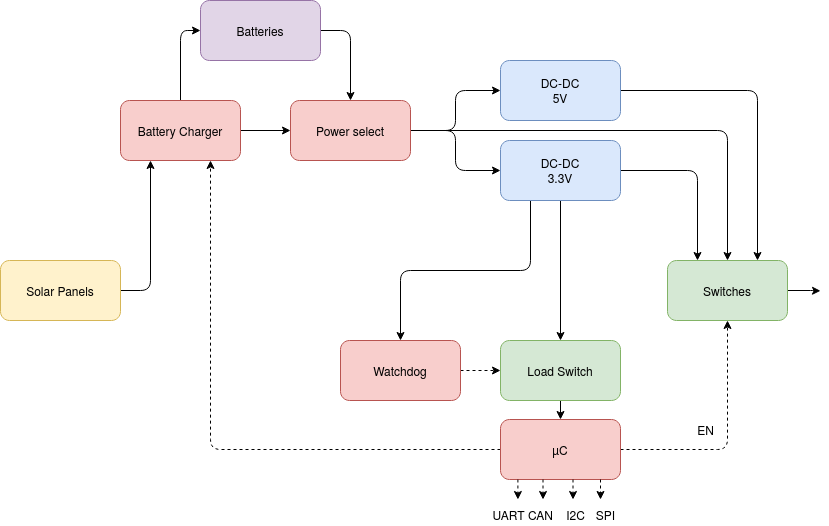
\includegraphics[scale=0.4]{EPS_basic.png}
			\caption{Example of the EPS Block Diagram}
			\label{fig: EPSS}
	\end{figure}

\subsection{Power Generation \label{sec:tech}}



Yost\cite{1} Solar power generation is the most used method for the nanosatellites to generate a power. Solar cells are build of thin silicon disks (semiconductor wafers)  which convert the energy of a light into electric current. Solar intensity of a solar array is light availability of the sun, which can vary according to a distance from the sun as well as angle of a projected surface area between the sun and a solar array.  
\\
\noindent\hspace*{3mm} Alia-Novobilski\cite{2} The most common manufactured type of cells are single junction cells. Single junction type is commonly used on the Earth applications. Due to severe sensitivity to a space radiation energy and relatively low efficiency, single junction type is not preferable for a space applications. Although single junction solar cell is relatively cheap to design, modern spacecraft use a multi-junction solar cells. Manufactured of a light-absorbing materials, multiple layers are much tolerant to a radiation in a space environment and more efficiently  Yost\cite{1} "convert specific wavelength regions of the solar spectrum into energy, thereby using a wider spectrum of solar radiation ". 
Green\cite{3} In the space industry, triple-junction solar cells are the most common tu use due to their high efficiency and relatively affordable cost compared to an other types of solar cells.

Fig. \ref{fig: GaAs} illustrates the example of a Triple Junction GaAs Solar Cell.

\begin{figure}[h]
	\centering
	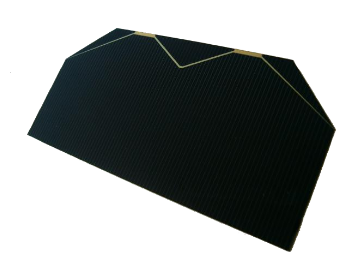
\includegraphics[scale=0.4]{azur.png}
	\caption{ 30\% Triple Junction GaAs Solar Cell \cite{4}}
	\label{fig: GaAs}
\end{figure}

Solar cells are usually interconnected to a solar array to get the desired power. Configuration of the solar array is flexible, such that it allows adjustment of the cells connection. To achieve the desired voltage, solar cells get interconnected in series (strings). To achieve the desired current, solar cells get interconnected in parallel.\\

\newpage

\begin{figure}[h]
	\centering
	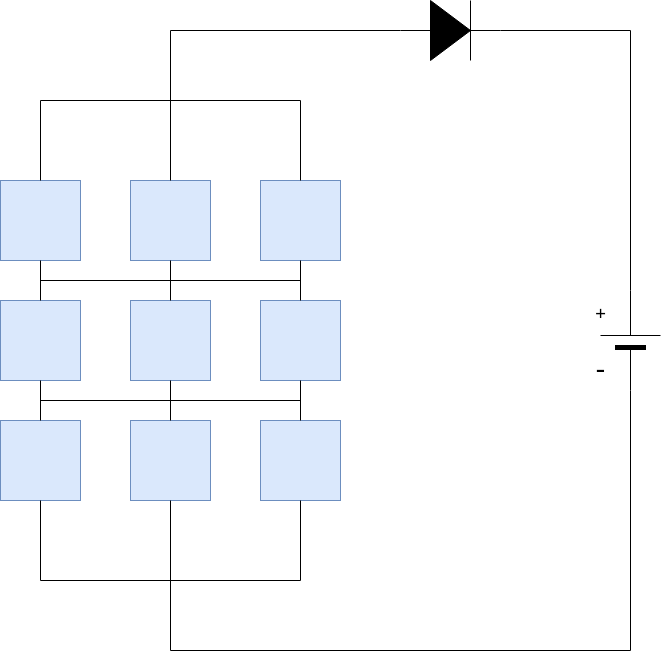
\includegraphics[scale=0.3]{Cellen.png}
	\caption{ Solar array}
	\label{array}
\end{figure}
	
Solar cell is strongly effected by a temperature. Honsberg\cite{5} "Increases in temperature reduce the band gap of a semiconductor, thereby effecting most of the semiconductor material parameters. The decrease in the band gap of a semiconductor with increasing temperature can be viewed as increasing the energy of the electrons in the material."\\
\\
Brieß\cite{6} The dependency of a temperature to the electric power of a silicon solar cell can be described as:\\ \\ \\

\begin{equation}
P = P_{ref} [ 1 - K_{P} ( T - T_{ref}) ]
\end{equation}
	\\
	\\
where:\\
     $P_{ref}$ - Power at reference temperature\\
     $K_{P}$ - Correction factor of power losses, 0.005$K^{-1}(for a silicon solar cell)$\\
     $T_{ref}$ - Reference temperature ( e.g. 25\textdegree{}C)\\
     
     

\begin{multicols}{2}
	\textbf{High  temperature:} \\ \\
	$\bullet$ reduce cell voltage \\
	$\bullet$ increase a cell current\\
	$\bullet$ reduce power\\
	

	\columnbreak
	
	\textbf{Low temperature:}\\ \\
	$\bullet$ increase cell voltage\\
	$\bullet$ reduce a cell current\\
	$\bullet$ increase power\\
	\\
\end{multicols}


	\begin{figure}[h]
		\centering
		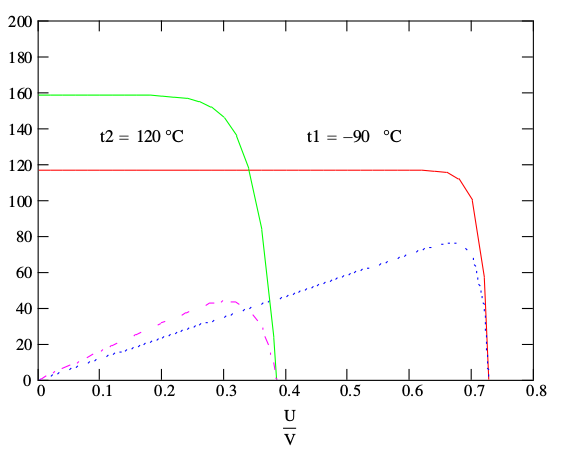
\includegraphics[scale=0.5]{temperatureDependancy.png}
		\caption{ Example of a solar cell characteristics at different temperatures\cite{6} }
		\label{fig: EPS11}
	\end{figure}
	
According to a Fig. \ref{fig: EPS11} a maximum power point shifts as a solar array getting hotter or colder. To keep power at the maximum point used Maximum Power Point Tracker (MPPT). The purpose of MPPT is to keep voltage on a particular level while solar panels are affected by a temperature or the orientation of the solar panels.\\
\cite{20} MPPT might be separated into two parts: power control, logic control. Power control is usually a step-up step-down DC-DC  converter which responsible for a voltage adjustment according to the input from the logic control. Logic control is responsible for a solar array parameters measurements and maximum power point adjustment according to the software algorithm.\\  

During the circuit design of the solar panels, it is important to consider the redundancy and a case in which one of the cells will be damaged. For that reason diodes are used. The diodes ensure the power can bypass a damage solar cell. Fig. \ref{dioden} illustrates the diodes D1 and D2 which are placed in the parallel with the solar cells. The diode D3 which can be also observed on the Fig. \ref{array} is used to prevent the reverse current. Reverse current has a negative effect on the solar panel efficiency. When reverse current occurs, it begins to draw current from the batteries, hence discharging them. In addition, reversed current adds additional current to the affected solar cell which shifts the maximum power point.\\


\begin{figure}[h]
	\centering
	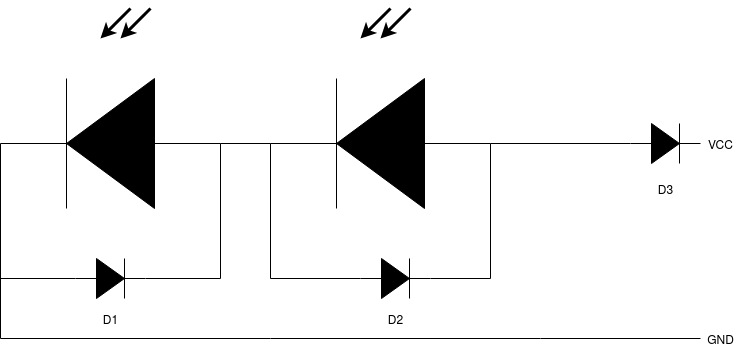
\includegraphics[scale=0.45]{DiodenSS.png}
	\caption{ Example of the Solar cell circuit design}
	\label{dioden}
\end{figure}
 
\newpage


\subsection{Power Storage \label{sec:tech1}}



Yost\cite{1} During the the mission duration, solar energy is not always available due to eclipse. For this case primary and secondary batteries used to store power. All batteries are classified according to their chemical characteristics. For a short mission duration (up to one week)  the primary type of batteries are usually used due to the lack of the possibility of recharging. The common chemical type of a primary battery is a silver-zinc, which is easier to handle, Yost\cite{1} "however there is also a variety of lithium-based primary batteries that have a higher energy density including: lithium sulphur dioxide (LiSO2), lithium carbon monofluoride (LiCFx) and lithium thionyl chloride (LiSOCl2)."\\
\\
Secondary-type batteries are rechargeable and provide an energy on demand. Secondary-type batteries are connected to a primary energy source of the satellite (usually solar panels) via battery charger. This type include: nickel-cadmium (NiCd), nickel-hydrogen (NiH2), lithium-ion polymer(LiPo), lithium-ion(Li-ion).

\subsubsection{Nickel Cadmium \label{sec:tech}}
 Buchmann\cite{7} Nickel Cadmium is a type of rechargeable batteries using nickel oxide hydroxide and metallic cadmium. This chemical connection allows battery to well perform by working in the savage conditions such as low or hot temperature. NiCd battery is the type which prefer to be charge fast instead of slow as types of secondary batteries. Full periodic discharge of a NiCd is an important process and necessary for battery performance. In case of absence  Buchmann\cite{7} " large crystals will form on the cell plates (also referred to as memory) and the NiCd will gradually lose its performance."
 
 \newpage

\begin{multicols}{2}

	\textbf{Advantages:} \\ \\
	$\bullet$ Big variety of size and performance options\\
	$\bullet$ Low price\\
	$\bullet$ One of the most robust rechargeable batteries\\
	$\bullet$ Good performance in the low temperature\\
	$\bullet$ Simple and fast charge\\
	$\bullet$ Big number of discharge cycles\\
	
	
	\columnbreak
	
	\textbf{Disadvantages:} \\ \\
	$\bullet$ Low energy density\\
	$\bullet$ NiCd has to be periodically discharged\\
	$\bullet$ NiCd contains toxic metals\\ 


\end{multicols}

Fig. \ref{fig: nicd} illustrates an example of the NiCd battery. 



\begin{figure}[h]
	\centering
	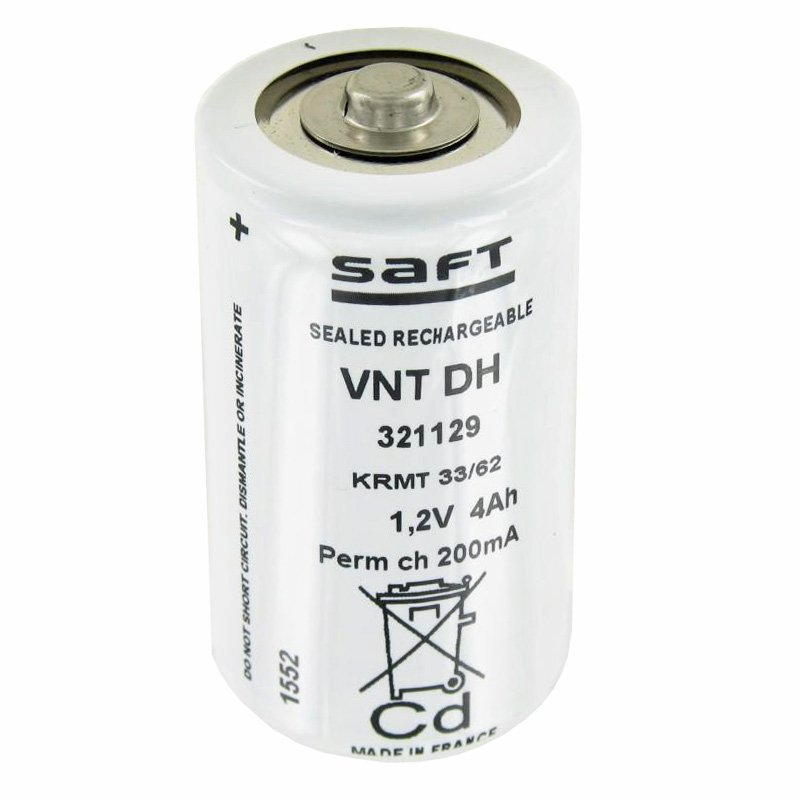
\includegraphics[scale=0.1]{NiCd.jpg}
	\caption{NiCd battery\cite{9}}
	\label{fig: nicd}
\end{figure} 


\subsubsection{Nickel Hydrogen \label{sec:tech}}
Buchmann\cite{7} Nowadays Nickel Hydrogen batteries are mostly used in the satellite applications where long time operation is required. The development of the NiH2 battery started in early 1970 year. In that time metal hybrid alloy was unstable, what slowed down development of the NiH2. In 1980 new alloy was established and stable enough to use it in the cell. 
\cite{10}"The replacement of cadmium with hydrogen electrodes has double the energy of Ni-Cd, but the specific energy of Ni- H2 is similar to Ni-Cd be case of the cylindrical configuration of the pressure. The first Ni- H2 battery was used in a GEO (geostationary mission) Intelsat V in 1983.  Almost all GEO spacecrafts now use Ni-H2 batteries. The first NASA LEO spacecraft to use Ni-H2 was in 1990."


Wenige\cite{8} Despite the fact that memory effect on NiH2 is undoubtedly less than on a NiCd batteries, it still exist and needs a special treatment in order to accommodate the normal level of the battery. Wenige\cite{8} "Typical calendar life of more than 20 years can be reached by NiH2, i.e. five years ground storage plus 15  years  orbital  life  in  GEO." \\ \\


\begin{multicols}{2}
	
	\textbf{Advantages:} \\ \\
	$\bullet$ High energy density\\
	$\bullet$ Environmentally friendly\\
	$\bullet$ Cheap\\
	$\bullet$ Less prone to memory effect\\
	$\bullet$ Suitable for a long life Satellite missions\\
	

	
	
	\columnbreak
	
	\textbf{Disadvantages:} \\ \\
	$\bullet$ Lose performance after deep discharge with high load\\
	$\bullet$ Requires long charge time due to heat generation\\
	$\bullet$ Require regular discharge to prevent memory effect\\ 
	$\bullet$ More expensive than a NiCd\\
	$\bullet$ Long life cycle

	
\end{multicols}

Fig. \ref{fig: nih2} illustrates an example of the NiH2 battery. 


\begin{figure}[h]
	\centering
	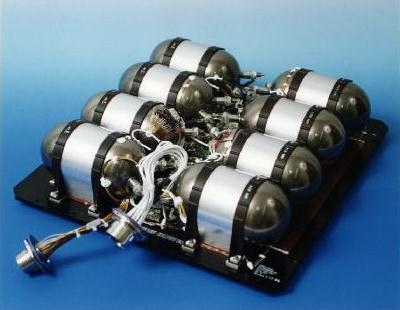
\includegraphics[scale=0.3]{NiH2.jpg}
	\caption{ NiH2 battery \cite{10}}
	\label{fig: nih2}
\end{figure}

\subsubsection{Lithium Ion \label{sec:tech}}

Buchmann\cite{7}Today lithium ion batteries is the most progressive and most promising batteries. Lithium is the lightest metal and able to provide the biggest energy density per weight. The energy density of a Lithium Ion batteries is about two times bigger then a NiCd. In addition, discharge characteristics of a Li-ion are similar to a NiCd, which offers a save utilization of a Li-ion batteries. Another advantage of a Li-ion batteries is a high cell voltage, which allows to allows to keep power properties with the light mass. Despite the fact that Li-ion batteries have many advantages, they also have their drawbacks. Li-ion batteries are very sensitive to an overcharge as well as an over discharge. For that reason Li-ion batteries usually used with protection circuits, which limit the peak voltage. In addition Li-ion batteries are prone to age even if not used Buchmann\cite{7} Over two or perhaps three years, the battery frequently fails.


\begin{multicols}{2}
	
	\textbf{Advantages:} \\ \\
	$\bullet$ High energy density\\
	$\bullet$ Low self discharge\\
	$\bullet$ No memory\\
	$\bullet$ High cell voltage\\
	
	
	
	
	\columnbreak
	
	\textbf{Disadvantages:} \\ \\
	$\bullet$ Require protection circuit\\
	$\bullet$ Aging without using\\
	$\bullet$ Does not apply for a long term use\\
	$\bullet$ Proper storage needed 

	
	
\end{multicols}

Fig. \ref{fig: lion} illustrates an example of the Li-ion battery. 

\begin{figure}[h]
	\centering
	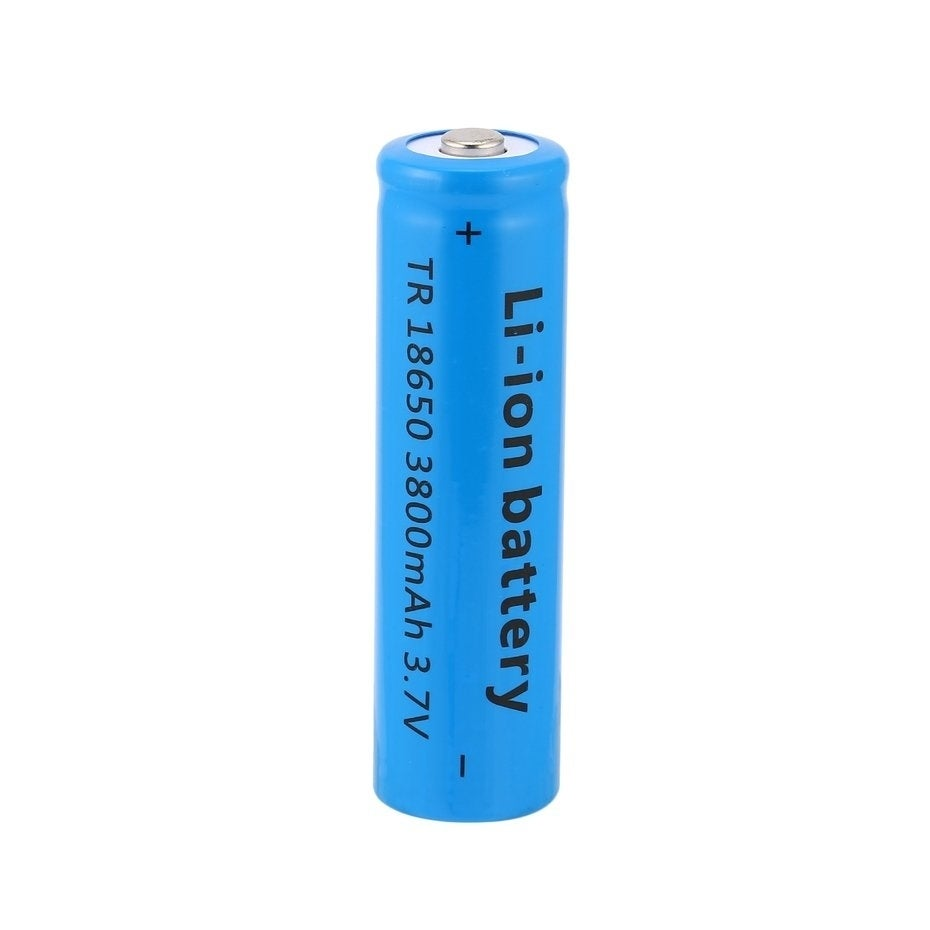
\includegraphics[scale=0.11 ]{Li-ion.jpg}
	\caption{ Li-ion battery \cite{11}}
	\label{fig: lion}
\end{figure}

\subsubsection{Lithium Polymer \label{sec:tech}}

In 1970, when the original design of lithium polymer batteries was invented, dry solid polymer electrolyte was used instead of  porous separator. Dry polymer design, allows to simplify manufacture process and the most important - to have a thin thickness geometry. However Dry solid polymer electrolyte experienced poor conductivity due to internal resistance of a the battery. Thereby, gelled electrolyte has been added to enhance ion conductivity. LiPo batteries have a slightly lower energy density and amount of charge/discharge cycles compare to Li-ion batteries. Nonetheless LiPo batteries have a bigger overcharge tolerance, which making them more robust to overcharge conditions.


\begin{multicols}{2}
	
	\textbf{Advantages:} \\ \\
	$\bullet$ Low profile \\
	$\bullet$ Flexibility to produce any shape\\
	$\bullet$ Weight\\
	$\bullet$ Resistant to overcharge\\
	
	
	
	
	\columnbreak
	
	\textbf{Disadvantages:} \\ \\
	$\bullet$ Lower energy density\\
	$\bullet$ Expensive\\
	$\bullet$ Does not apply for a long term use\\
	$\bullet$ Proper storage needed 
	
	
	
\end{multicols}

Fig. \ref{fig: lipo} illustrates an example of the LiPo battery. 

\begin{figure}[h]
	\centering
	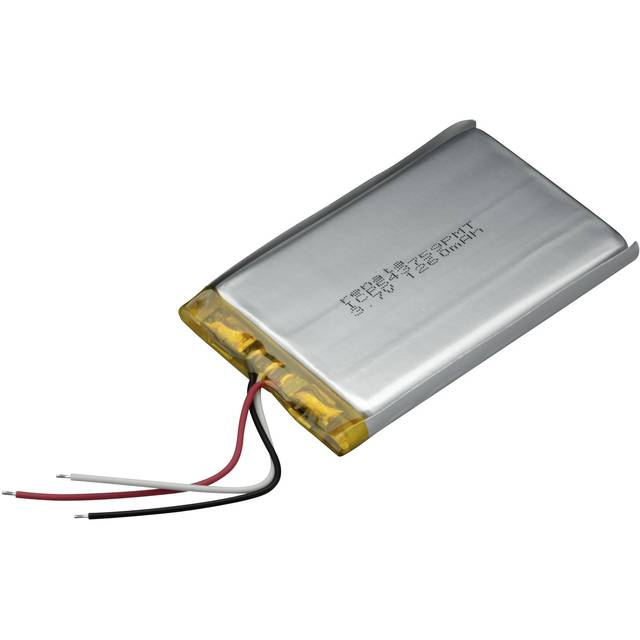
\includegraphics[scale=0.16]{LiPo.jpg}
	\caption{ LiPo battery \cite{12}}
	\label{fig: lipo}
\end{figure}



\subsubsection{Charging}

Santoni\cite{13}The hight capacity and low weight make Li-ion batteries very well suited for a nanosatellite space applications. Nonetheless performance and safety charging issues should be taking into account. Insidor\cite{14} The charge of a LI-ion batteries is very strict on the correct settings, mostly due to a high sensitivity to a overcharge. Typical Li-ion battery voltage per cell can vary from 4.1 to 4.3, which is defined in the datasheet. However, typical and most common value is 4.2V. Exceed of a battery voltage limit will increase capacity, but will also stress a battery, which can seriously harm a cell and and significantly reduce battery performances.\\ \\
Li-ion/Po battery charge process can be divided into 2 main stages:\\
$\bullet$ constant current charge\\
$\bullet$ constant voltage charge\\

Fig. \ref{fig: bcs} illustrates the example of battery charging stages.

\begin{figure}[h]
	\centering
	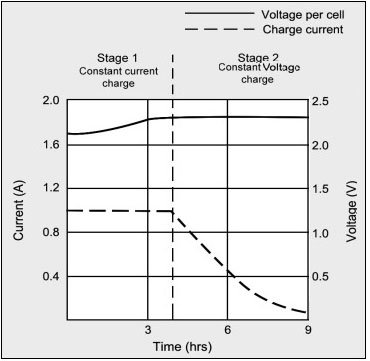
\includegraphics[scale=0.7]{bcs.jpg}
	\caption{ Charge stages \cite{14}}
	\label{fig: bcs}
\end{figure}
 Charging rate of a battery measures in C. In case of 1000mAh battery cell 1C charging rate will be 1000mA and 500mA for 0.5C. Usually, recommended charging given in the datasheet.\\
 Charging process starts with a 100\%  constant current (according to a charging rate) process. During the time while battery voltage reaching the upper voltage threshold, its pushing a constant current into a battery. Once voltage reaches threshold point, charging process changes from the constant current mode into a constant voltage mode. In a constant voltage mode, voltage keeps its maximum level while current starts to slightly drop until it gets down to a threshold level, which usually written in a datasheet (around 3\%). After current drops below the threshold, battery is fully charged. \\ \\
 In most cases, IC chargers are used to provide constant current and constant voltage for lithium-ion / Po batteries. \cite{14} One of those IC chargers is a MAX745. 
This IC is able to set a charge up to 4 cells in series, as well as set a current and charging voltage. This IC use PWM signal to control a charge voltage which does not allow IC to get too hot.\\ This IC is an example of a charger microchip which has all necessary  tools to charge a Li-ion/Po batteries. 



\begin{figure}[h]
	\centering
	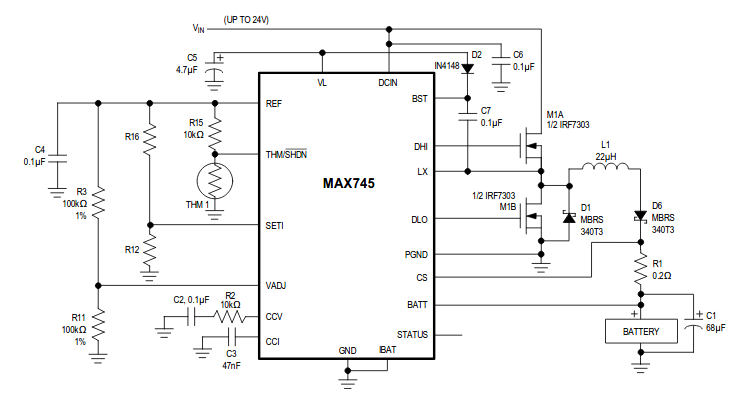
\includegraphics[scale=0.5]{MAX745.png}
	\caption{ Li-ion/Po charger MAX745 \cite{15}}
	\label{fig: EPS22}
\end{figure}

The Figure \ref{fig: EPS22} shows an example of a standard MAX745 application circuit. On the left side of the schematics pins SETI and VADJ are used to adjust a charge voltage and charge current. External resistors R16,R12 are connected to a reference voltage to adjust a charge current and resistors R3,R11  used to adjust charge voltage. On the right side of the schematics MAX745 use two external N-channel MOSFETs which control power from the input source which controlled by current mode, PWM controller. 



\subsubsection{Protection}

Despite the fact that, Lithium-ion/Po batteries have a high density, they also require a careful handling. For this reason, it is important to use protective circuits that prevent overcharging, over-discharge and quick discharge of Li-ion batteries.\\
\cite{16} Overcharge of a Li-ion/Po batteries case an immense battery stress which creates a safety hazard with a possibility of fire. Li-ion batteries have a less tolerance to an overcharge and require a protection circuit.\\
The over-discharge of a Lithium batteries is also harmful. The consequence of over-discharge is a reduced battery life, due to the dissolution of copper from the anode into the electrolyte, which can case a short circuit during a battery charge.\\
Protection ICs used to comply all upper mention conditions. A main principal of a protection IC is to switch on and off a power line usually by using external MOSFETs to keep a batteries safe and not exceed a voltage threshold. The simple example of a protection IC is a BQ29700D which is a one cell protection device. 

\begin{figure}[h]
	\centering
	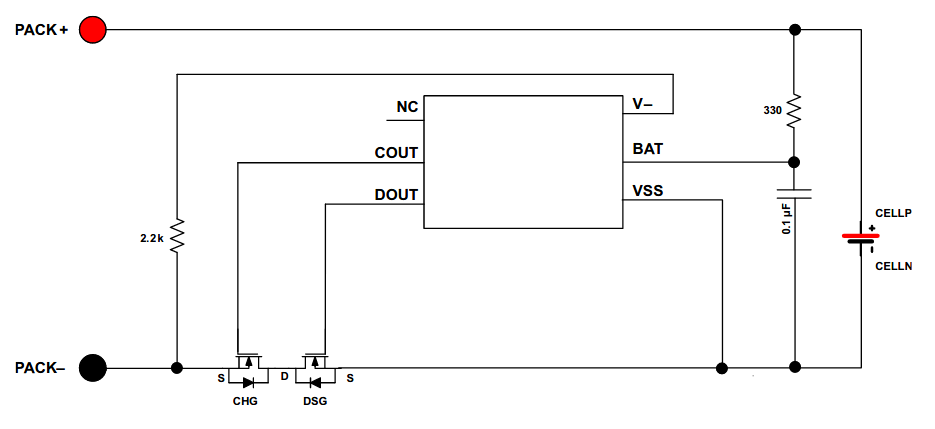
\includegraphics[scale=0.5]{protect.png}
	\caption{ BQ29700D protection IC \cite{17}}
	\label{fig: EPS1}
\end{figure}

Figure \ref{fig: EPS1} illustrate a typical schematics of a protection circuit where BQ29700 connected with two MOSFETs defined as CHG and DSG, and a battery cell. In case of overcharge detection, COUT pin pulls a CHG MOSFET which disconnect ground line and stops charging process. In case ocer-discharge detection, DOUT pin pulls a DSG MOSFET which dissconect ground line and stops discharging process of a battery.

\subsection{Power processing \label{sec:tech}}

Power processing is an important part of an EPS which is responsible for transforming voltages to be suitable for satellite subsystems and payloads. Nowadays there are many converters available; each type has it's own advantages and disadvantages. Hemmo\cite{18} A converter has to be chosen according to subsystem requirements such as voltage range, maximum power output, output voltage tolerance, efficiency and footprint. The power efficiency of a converter is a very important criterion of stored energy due to the fact that battery energy is limited. High efficiency of  power conversion reduces the power dissipation of  components, thereby decreasing the power consumption if batteries. Furthermore, the need for any heat sinks is reduced or altogether eliminated. 

\subsubsection{Linear Voltage Converters \label{sec:tech}}

Hemmo\cite{18} One of the oldest methods to convert a power is a linear voltage conversion. This method based on power dissipation into a resistor, which case a voltage drop. Power dissipation of a linear voltage converter can be calculated by using formula:\\ \\

\begin{equation}\label{eq:2}
P_{diss}=U_{drop} \times I
\end{equation}


where:\\
$U_{drop}$ - resistor voltage drop\\
$I$ - current through a resisor\\ \\
 Tietze \cite{18} Linear voltage conversion is a simple method, which does not require many additional passive components, relatively cheap and easy to use. Nonetheless due to a power dissipation linear voltage converters are getting hot, which make them ineffective while current through a resistor is large or difference between $V_{in}$ and $V_{out}$ is high according to \eqref{eq:2}. For that reason Linear voltage converters used only in case of low current and low voltage drop for example to convert power into a micro controller or to provide a voltage reference.\\
 \\
 
 
\subsubsection{Inductive DC-DC Converters \label{sec:tech}}

Tietze\cite{18} Each inductive DC-DC converter consist of three passive components: inductor $L$, power switch $S$ and capacitor $C$. The use of these components in various topologies, allow to create various types of DC-DC converters such as a step-down converter where output voltage $0 \leq U_{a} \leq U_{e} $ , step-up converter where output voltage $U_{a} \geq U_{e} $  and   step-down step-up converter which is able to decrease and increase output voltage, for this type of a converter $ U_{a} > 0$. Use of inductive DC-DC converters offer better efficiency due to switching power supply, which gives an advantage over the linear voltage regulator. Hemmo\cite{17} High efficiency is extremely required parameter for a space application due to the limited power generation. In addition, inductive DC-DC converters are able to produce  voltage output $U_{a}$ which is higher then voltage input $U_{e}$. Inductive DC-DC converters used in most cases in the aerospace industry due to high efficiency and capability to manage high voltages and high current.

\begin{figure}[h]
	\centering
	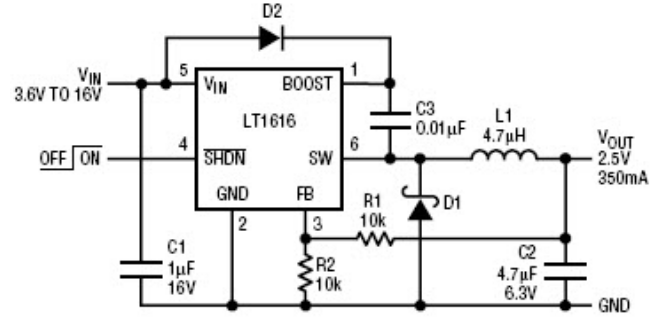
\includegraphics[scale=0.4]{ltc1616.png}
	\caption{ Inductive DC-DC converter \cite{19}}
	\label{fig: EPS41}
\end{figure}

Figure \ref{fig: EPS41} illustrates an example of the simple Inductive DC-DC step-down converter LT1616. The inductor L1 allows peak current to be reduced in order to not harm the C2 capacitor and to store the energy while the inner switch is closed. The diode D1 provide a different path for the current while inner switch of the LT1616 is open. The output voltage of converter can be programmed by choosing a value for the resistors $R1$ and $R2$ according to a formula from the datasheet \cite{19} . 
\\
\\

\subsection{Microcontroller \label{sec:tech}}
The main responsibility of the EPS microcontroller is to manage a power distribution for a hole satellite by sending an enable signals to a commutating components, in most of the cases integrated switches. In addition, microcontroller provide a housekeepeng telemetry by reading the values of sensors, such as temperature sensors, current sensors and others. For this task EPS microcontroller uses protocol lines as $I^{2}C$ or $SPI$. Furthermore, EPS microcontroller needs to communicate to an OBC microcontroller to share the housekeeping information or for reason to receive a commands from OBC. Communication between EPS and OBC as well as with other microcontrollers implemented via CAN bus. Moreover, EPS microcontroller can be used to handle MMPT algorithm to obtain the maximum power from the solar energy. The example of microcontroller block diagram architecture shown on the Fig \ref{fig: EPS4121}.	
\\
\begin{figure}[h]
	\centering
	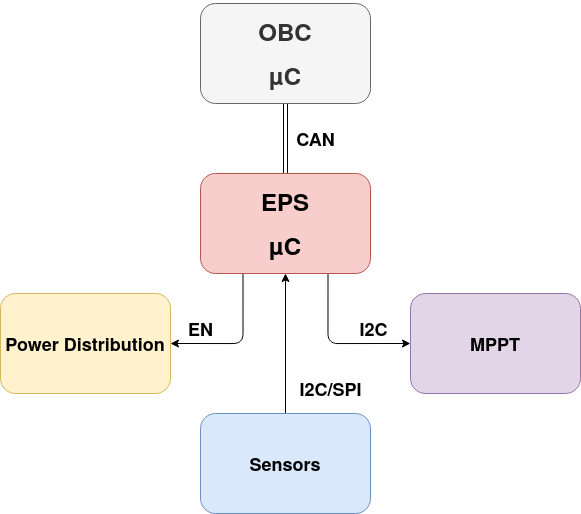
\includegraphics[scale=0.4]{uC.png}
	\caption{block diagram of microcontroller communication}
	\label{fig: EPS4121}
\end{figure}
\\
EPS Data signals:\\ \\
$\bullet$ CAN\\
$\bullet$ UART\\
$\bullet$ I$^{2}$C\\
$\bullet$  SPI\\
$\bullet$  EN\\
\\
As for power consumption, microcontrollers consume very little power. Some microcontrollers such as STM32L  can consume  around 10 to 100 $\mu$A.\\
To prevent the microcontroller of getting stuck, external watchdog is used. Watchdog receives the signal from the microcontroller which restart the timer. If case that watchdog did not receive a signal, he will send a signal to a load switch, which will restart the microcontroller by turning the supply power "OFF" and "ON".

\subsection{Power Distribution \label{sec:tech}}

Power distribution is a vital part of the EPS, needed to \cite{21} "supply electrical power to the subsystems and payloads of the satellite" as well as prevent an overload of the main power bus. Power distribution usually consist of load switches which distribute power with help of microcontroller by sending the enable signal to an appropriate pin of the switch. In addition, current sensors are used to monitor the payload or power consumption of the subsystem. This combination allows to fully control the process of power distribution. Figure \ref{fig: EPS111} illustrates an example of the EPS power distribution where $R_{sense}$ is a shunt resistor for a current sensor. 


\begin{figure}[h]
	\centering
	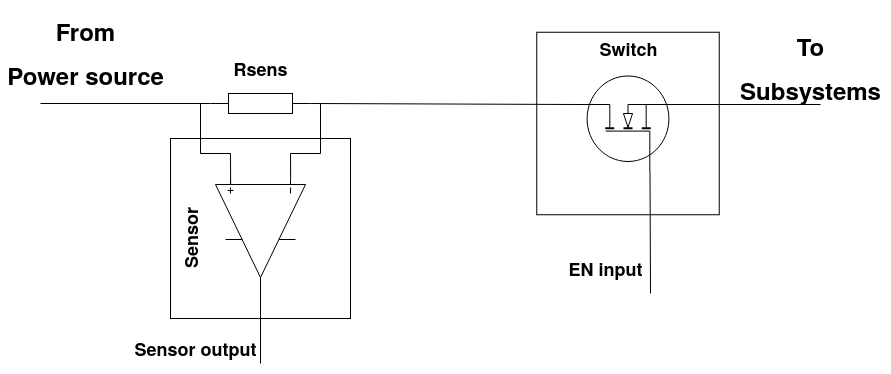
\includegraphics[scale=0.35]{distrib.png}
	\caption{Power distribution with power switch and current sensor}
	\label{fig: EPS111}
\end{figure}

\newpage

\subsubsection{Switches}
Power distribution include load switches which responsible for a power commutation of a satellite. Power switches are integrated chips which designed for specific cases and scenarios. One of the important parameters is a power load. Switches have to be chosen according to a load of a power lines considering voltage and maximum current. Otherwise, if the input power exceeds the power that the switch can operate with, this might lead to destruction of the switch and the entire power line.  Another aspect which has to be considered is the inrush current. Inrush current is a maximal instantaneous current draw by an electrical device, appeared for few microseconds when first turn on. Inrush current cased a voltage drop for the supplied subsystems, which might harm device or case incorrect device performance.

 Capacitors might be used to prevent inrush current. The value of capacitor has to be calculated by equation \ref{eq:3} \cite{32}:
 
 \begin{equation}\label{eq:3}
 C_{L} = I_{INRUSH} \times \dfrac{dt}{dV_{out}}
 \end{equation}
 
 Where:\\ \\
 $I_{INRUSH}$ - amount of inrush current\\
 $C_{L}$ - Value of capacitor \\
 $dV_{out}$ - maximum allowable voltage drop\\
 $dt$ - rise time\\

Another important ability of the switcher is the fault detection. Fault detection appear while current on the power line exceed the programmed current of the switch. Whilst Overcurrent was detected, switch sends a signal to a microcontroller to disable the switch. Fault detection often used to detect Lautch-up of the satellite.\\

\subsubsection{Power Monitoring}

Power monitoring is the necessary part of the EPS, which allows to observe the current status of each subsystem and payloads of the satellite. \cite{22} "Power monitoring is implemented by measuring the 
voltage drop across a shunt resistor.  The voltage across the shunt  is  usually  amplified  using  a  differential amplifier" and produce the analog output. Nowadays Current sensor ICs used to monitor a current on the power lines. Modern current sensors have ability to output measured information as I$^{2}$C or SPI data by converting an analog output signal to the digital via integrated analog to digital converter. 

\newpage   
\chapter{6 Unit Satellite Design \label{chapter3}}
This chapter will provide a short essential knowledge about Descartes Mission with the main purposes of the mission, satellite characteristics and the satellite  abilities. Then topic will go deeper into the EPS architecture design of the 6U satellite. \\
\section{Introduction into the Descartes Mission}

German Orbital System (GOS) plays a major role in the satellite development. GOS has accomplished nine successful 3U satellites launches into space since their realize as a company. Although 3U satellites are relatively cheap to build and their characteristics enough have a simple payload, GOS is keeping up with the time. At the moment GOS is developing the 6U nanosatellite (Descartes), that shown on the Figure \ref{fig: EPS222}. Descartes can be used for a wide range of tasks such as:\\ \\
$\bullet$ Earth exploration\\ 
$\bullet$ Student projects\\ 
$\bullet$ Science projects\\ 
$\bullet$ Orbit calibration and control\\ 
$\bullet$ Auto Dependent Surveillance Broadcast\\ 



\begin{figure}[h]
	\centering
	\includegraphics[scale=0.19, angle =90]{descart.png}
	\caption{The Descartes satellite}
	\label{fig: EPS222}
\end{figure}


  Descartes is a 6U satellite with dimensions 360$\times$240$\times$120 and mass less than 8kg. 6U satellite has 3.5U of payload free space, which is reserved for the four different payloads. Descartes developed for a 2 years of lifetime on the Low Earth Orbit. For his orbital lifetime satellite will measure the space weather, observe the aircrafts, monitor the ultraviolet radiation on the Earth atmosphere  and provide remote sensing of Earth. The Space weather measurements implemented by DeCor payload. DeCor is a detector of gamma radiation and charged particles in the range of 0.3-3 MeV.This device allows to study the fast variations of electron fluxes in the gap zone between radiation belts and dynamics of particle fluxes and gamma radiation in low orbits depending on geomagnetic conditions. Aircraft data are monitored using a payload called AMUR. AMUR is designed to collect, process and filter aircraft data. 
  In addition to having a four different payloads, Descartes is using 3-axis attitude control which consist of reaction wheels, magnetorquers and sets of magnetic and solar sensors. To transmit the telemetry and commands Descartes use 2 UHF modules which were designed ba GOS. In addition to 2 UHF modules, 6U satellite operate with a 2.4 GHz HISPICO S-band transceiver.\\ \\
 
 
  \section{EPS Architecture of the 6U Satellite}
  According to an introduction into the mission it is noticeable that design of the 6U satellite highly improved in comparison with the previous 3U satellites which were designed by GOS. The biggest divergence is a size and availability of the satellite to work with more payloads as well as to perform 3-axis stabilization. Due to that fact, the EPS of the satellite has also undergone changes.
  
  Due to the energy requirements, 6U satellite has to provide a 160 Wh of energy and  distribute it to 23 channels. To accomplish this requirements, considering the available space of the 6U satellite, EPS was devided into 3 main parts which connectrd between each other via PC104 connector:\\ \\
  $\bullet$ Power Proccessing Unit\\
  $\bullet$ Power Distribution Unit\\
  $\bullet$ 2 Battery Packs\\
  
   \subsection{Power Processing Unit}
   PPU is a part of EPS which responsible for a battery charge, power distribution control and a power processing. The PPU is illustrated on the Fig. \ref{fig: psu122}.
   
   \begin{figure}[h]
   	\centering
   	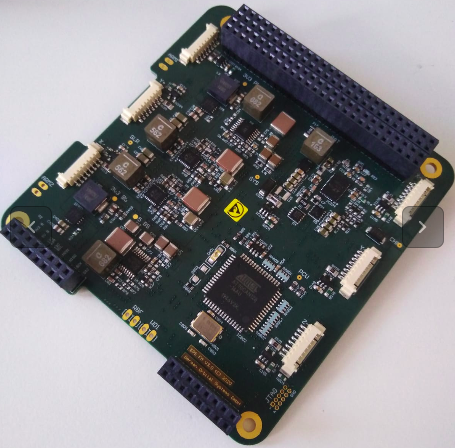
\includegraphics[scale=0.4]{ppu.png}
   	\caption{PPU}
   	\label{fig: psu122}
   \end{figure}
   
   Power converted from the solar flux come first into a PPU from 6 solar panels: X+, X-, Y+, Y-, Z+, Z-. At first, input power of each solar panels gets measured by MAX7328 current sensor. Then power goes into a microchip LTC4015 which is responsiable for a battery charge, illustrated on the Figure \ref{fig: ltc40151}. Integrated circuit LTC4015 provide a constant voltage and current into a batteries at the same time passing unregulated power from the solar panels directly into a system load. Although LTC4015 can be adjusted for a battery charge manually, microchip might use an MPPT algorithm to regulate the voltage in order to keep maximum power peak. This allows to charge and discharge the batteries according to a batteries state of charge and solar condition (eclipse). Microchip draws power from the solar input to the system, while batteries are charging and switch power source to a battery pack while eclipse or overcharge condition.
   
  \begin{figure}[h]
  	\centering
  	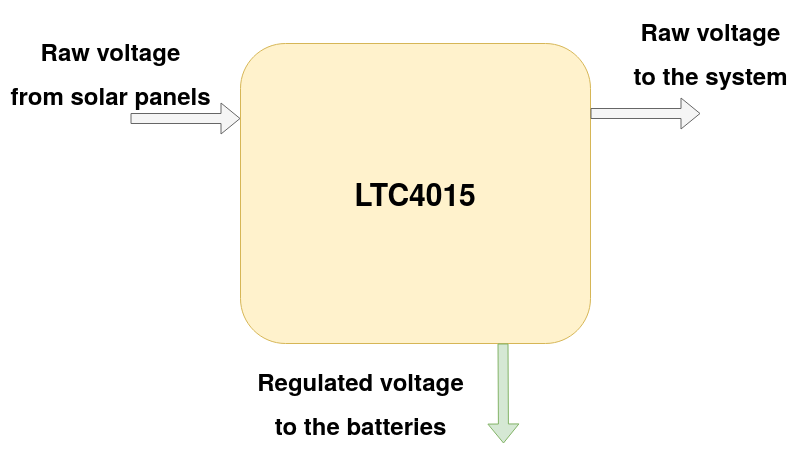
\includegraphics[scale=0.2]{ltc4015.png}
  	\caption{Battery charger}
  	\label{fig: ltc40151}
  \end{figure}
  
 After the power has been distributed from the charger, is separates in two power lines, one power line goes through the LDO converter to feed the microcontroller and second distributes the power into five DC-DC converters for the subsystems and payloads.
 
 LDO converts input power from the charger into 3.3V to supply a power for microcontroller. After surpassing the LDO, power goes through the load switch, controlled by watchdog. Watchdog provide a constant output signal to the load switch, that alloud him to commutate and transfer power further to the microcontroller. 
  
    \begin{figure}[h]
    	\centering
    	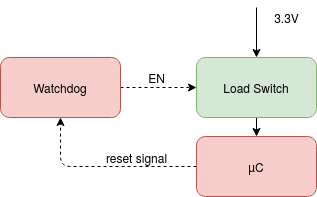
\includegraphics[scale=0.7]{Watch.png}
    	\caption{microcontroler power supply}
    	\label{fig: ltc4015}
    \end{figure}
  Microcontroller sends a reset signal to the watchdog, to to reset the counter. As long as counter reset, watchdog keep the enable output pin "HIGH". However, when watchdog does not receive the reset signal from the microcontroller due to some system problems, watchdog restart himself and enable output pin getting low and high, which restart microcontroller.
  
  5 DC-DC converters of the PPU convert the input power from the LTC4015 charger. Power processing can be divided into 2 blocks power processing for the BUS and power processing for the payload. Each block has 2 DC-DC step down converters, 5V, 3.3V and one common 7.4V. Common 7.4 V converter used to convert unregulated voltage from the solar panels. For this task LTC3119 used, this microchip has a big current tolerance which allows him to transfer huge amount of power.To produce 5V and 3.3V, used LM43603 and TPS62111 converters. This converters were successfully used on the previous EPS models. In order to keep a flight heritage, were made decision to keep the converters as it is. 
  
   \begin{figure}[h]
   	\centering
   	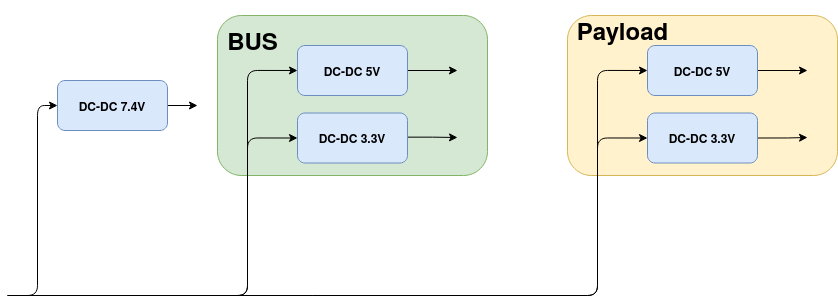
\includegraphics[scale=0.4]{dcdc.png}
   	\caption{Power processing}
   	\label{fig: ltc4015}
   \end{figure}
  
  One of important tasks of the EPS and PPU is to deploy 2 UHF antennas. To accomplish this task and provide a battery voltage to deployment mechanism, used 2 power lines for each UHF antenna with two TPS1H200A load switches in series for each line. To activate antenna release, two signals must be send from the microcontroller which enable the load switch to commutate and provide a power to accomplish antenna release on the Fig.\ref{fig: PPU} antenna release mechanism shown as ARM1 and ARM2. 
  
  In addition, PPU provide a current and voltage sensing of 16 analog lines,  which get converted via ADC MAX1231 that provide an SPI signal. 
  
  Figure \ref{fig: PPU} Illustrate the simple PPU architecture block diagram. 
  
  \begin{figure}[h]
  	\centering
  	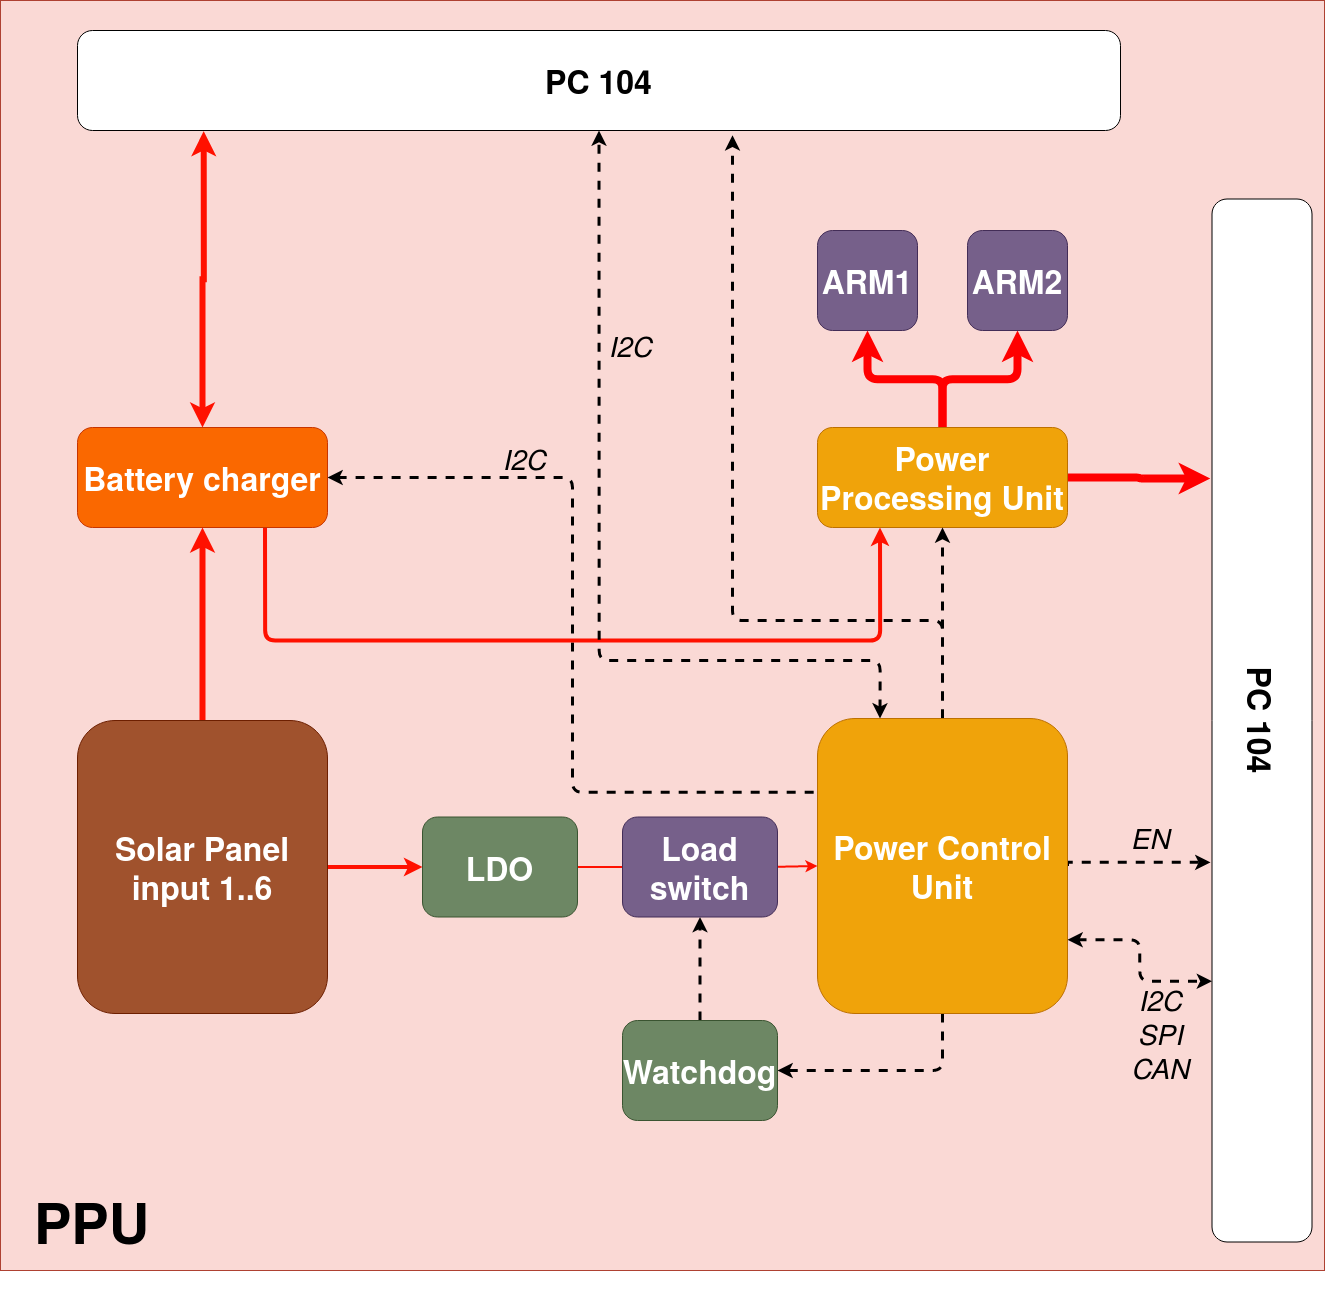
\includegraphics[scale=0.3]{PPU.png}
  	\caption{Power Processing Unit}
  	\label{fig: PPU}
  \end{figure}
  
     \subsection{Battery Pack}
  
 Battery pack board used to provide a power storage for the EPS by using of 4 li-ion batteries with a 2 series 2 parallel configuration. One of the EPS requirements is to provide capacity of 160 Wh which can be made by using 2 battery packs with LI-ion batteries samsung INR21700 with a capacity of 4900mAh.
 
 \begin{figure}[h]
 	\centering
 	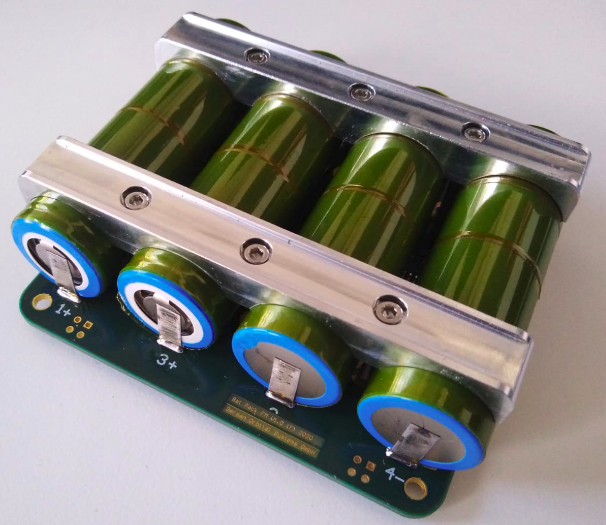
\includegraphics[scale=0.37]{bat.png}
 	\caption{Battery pack board}
 	\label{fig: bat}
 \end{figure}
 
  As was discussed in the background section \ref{sec:tech1} Li-ion batteries required a protection circuit to prevent overcharge, over-discharge and a fast discharge(short). For the battery pack board every two cells in the series have their own protection integrated chip BQ29700D which has an overcharge, over-discharge and short protection. Due to 2S2P configuration, batteries which located in parallel have to be balance. BQ29209 is a battery balancer from Texas Instruments which \cite{23}"performs automatic cell-balance correction where the two cells are automatically corrected for voltage imbalance by loading the cell with the higher voltage with a small balancing current."  
  
  \begin{figure}[h]
  	\centering
  	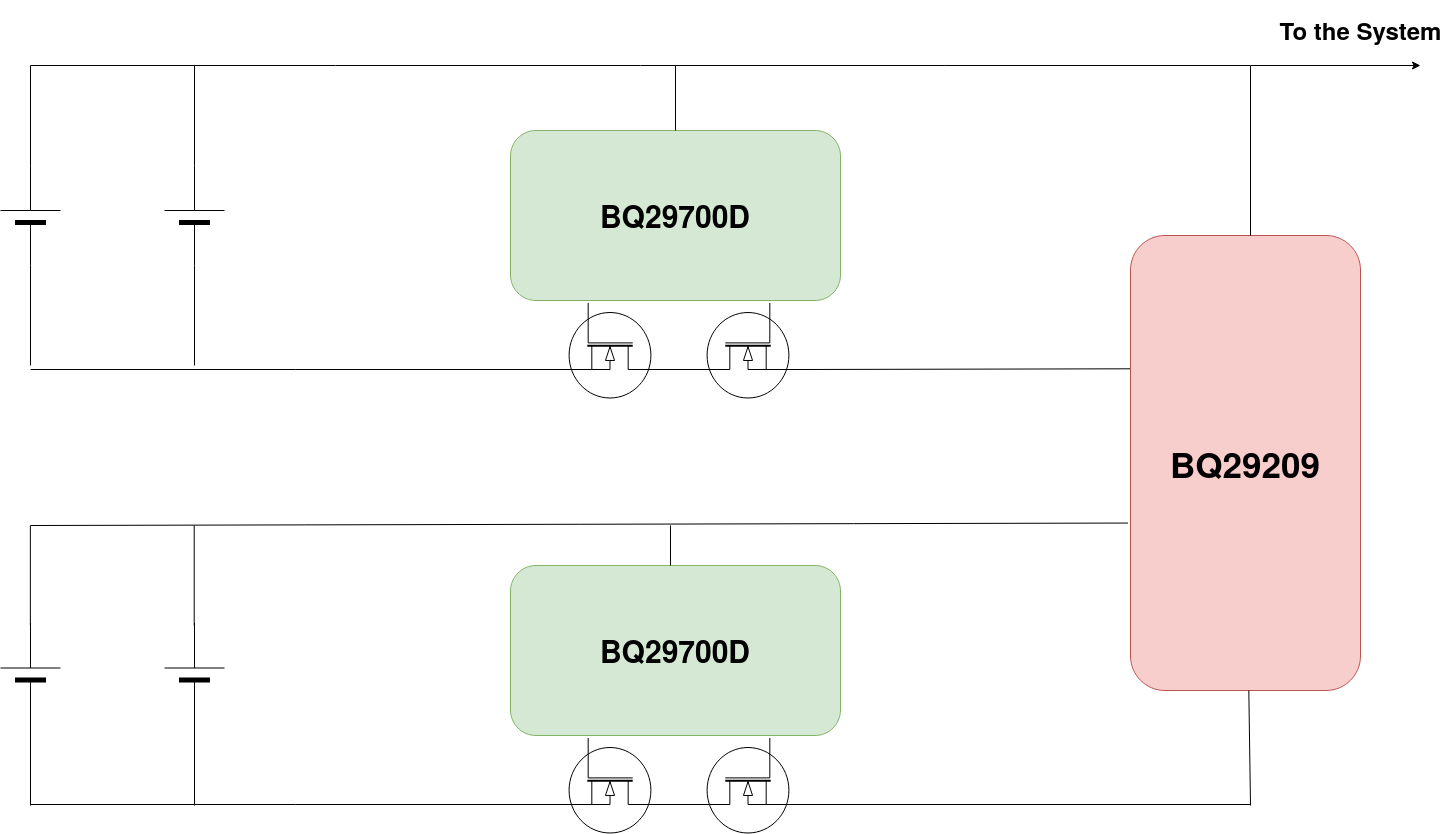
\includegraphics[scale=0.2]{2s2pMasterarbeit.png}
  	\caption{Battery protection-balancing}
  	\label{fig: Bat_prot_bal}
  \end{figure}
  
  The configuration \ref{fig: Bat_prot_bal} allows batteries to provide and collect the power at the same time keeping cells balanced and safe.
  
  Due to the space environment, temperature of the batteries can decrease bellow the temperature threshold. To avoid the battery temperature drop bellow the limit, was decided to use resistor heaters. Battery pack board has 2 temperature sensors that located under the batteries, which allow to measure the temperature close to the temperature of the batteries. The temperature sensors provide an I$^{2}$C to the PC104 connector that transfer the data signal to the microcontroller of the PPU. Microcontroller reads the signal and decide whether it need to provide a heat to the batteries or not. Heat is implemented by sending a enable signal from the microcontroller to the load switch TPS1H200A that has a function to transfer a power from the batteries to the low value resisters.  \\ \\ \\ \\
  
  
  \begin{figure}[h]
  	\centering
  	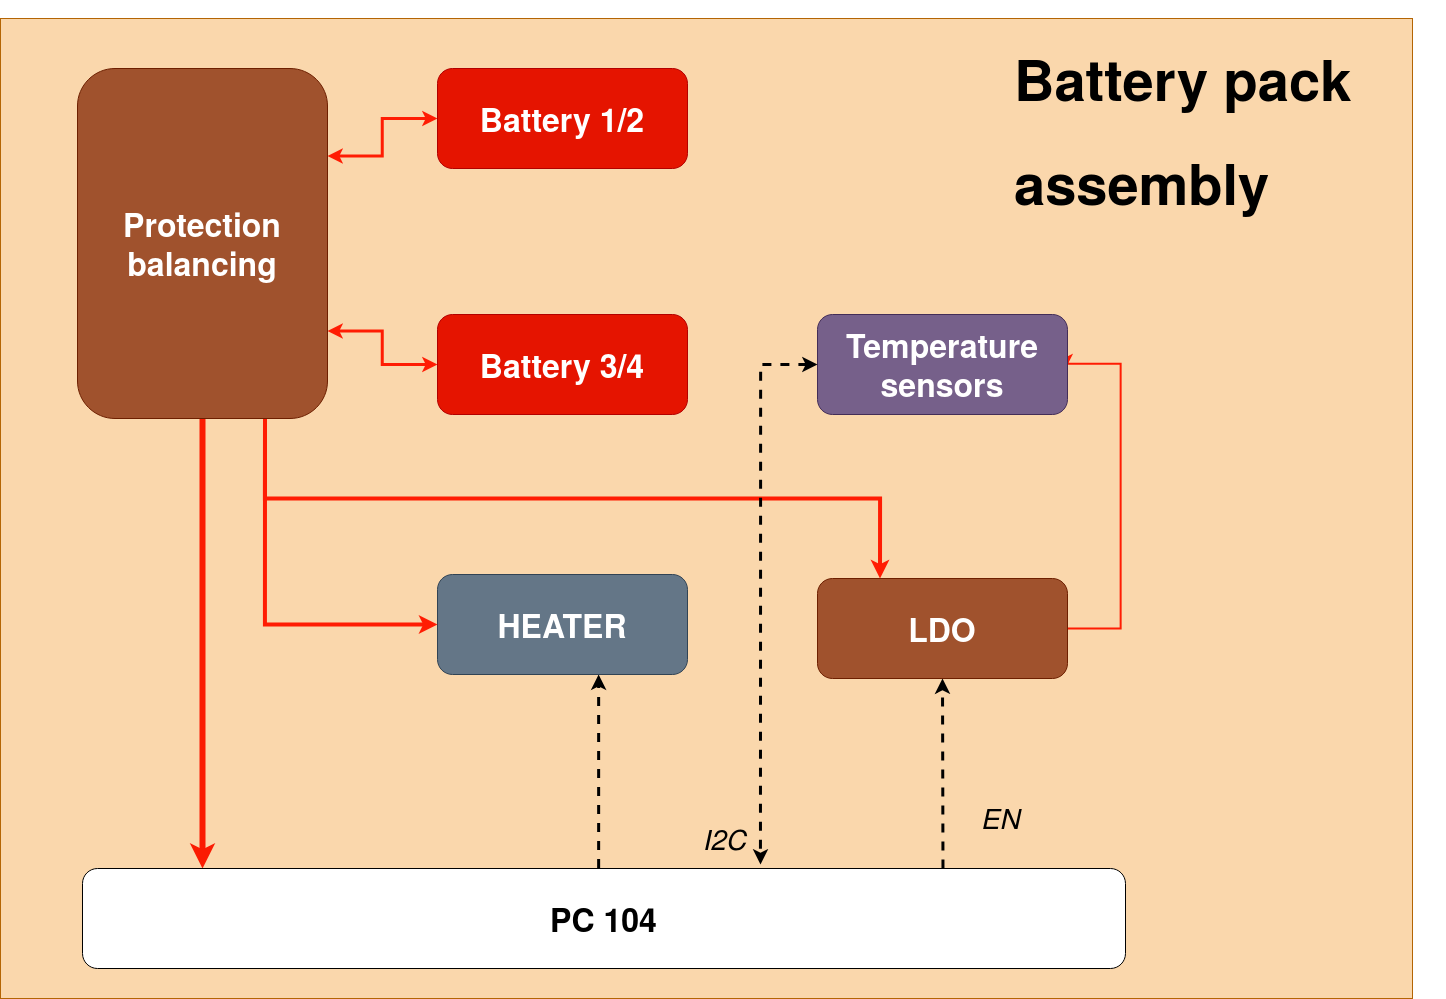
\includegraphics[scale=0.3]{BP.png}
  	\caption{Battery pack board}
  	\label{fig: BP}
  \end{figure} 
   
  
  \subsection{Power Distribution Unit}
  PDU is a part of the EPS that responsible for a power distribution and power monitoring. The main feature of PDU is the flexibility, that allows the PDU to fit every power requirement of the subsystem or payload.     To provide a power to the subsystems and payloads PDU uses 23 load switches of 3 different types TPS203x, TPS1H200A and FPF2701. The power distribution is controlled via EPS microcontroller by providing an enable signal to the pinhead connectors and partly by transmitting an I$^2$C signal to shift register that spread an array signal into the switches. 
  
  In order to measure a current of the power lines to observe a power consumptions of the subsystems and payloads, MAX4372 is used. Current sensors located one for each power line, which allows to measure the current of each line. MAX4372 has an analog output, which requires to use an ADC converter to convert an analog into a digital signal. To convert analog into a digital signal was decided to use MAX1231 ADC converter that provides an SPI output signal to the EPS microcontroller. 
  
    
  The detailed review, calculations and all explanations of the PDU board will be given in chapter \ref{sec:tech77}
  
    
  
    

    
  

  
  
  


    \chapter{Requirements\label{cha:chapter3}}

\section{Top Level Requirements}
The PDU shall be able to provide sufficient power to fulfill requirements of subsystems and payloads using common regulated voltages 3.3 V, 5 V and regulated battery voltage 7.4V. Top level requirements are given by GOS specially for the Descartes Mission. There are 22 top level requirements which are shown in the Tab. \ref{Tab:req1}. 

\captionof{table}{PDU Top Level Requirements}
\begin{longtable}{p{1cm}p{11cm}p{2cm}} \toprule
	ID & Description & Verification \\ \midrule
	

	

TL1 & PDU shall provide the AURA experiment a 5V line & Test\\
TL2 & PDU shall provide the AURA experiment up to 3W during operations & Test\\
TL3 & PDU shall provide the Decor experiment a 7.4V line & Test\\
TL4 & PDU shall provide the Decor experiment up to 0.2W and 0.8W respectively & Test\\
TL5 & PDU shall provide the AMUR experiment a 5V line & Test\\
TL6 & PDU shall provide the AMUR experiment up to 0.2W during operations & Test\\
TL7 & PDU shall provide the OBC a 3.3V line & Test\\
TL8 & PDU shall provide the OBC up to 0.42W during operations & Test\\
TL9 & PDU shall provide the LoRa a 5V line & Test\\
TL10 & PDU shall provide the LoRa a 1W during operations & Test\\
TL11 & PDU shall provide the ADCS 5V and 3.3V respectively & Test\\
TL12 & PDU shall provide the ADCS up to 2.3W and 0.2W respectively & Test\\
TL13 & PDU shall provide the UHF 7.4V line & Test\\
TL14 & PDU shall provide the UHF up to 5.2W during operation & Test\\
TL15 & PDU shall provide the HISP 5V line & Test\\
TL16 & PDU shall provide the HISP up to 7.5W during opertaion & Test\\
TL17 & PDU shall provide the ARM a 5V line & Test\\
TL18 & PDU shall provide the ARM up to 10W during the release & Test\\ 
TL19 & PDU shall provide CAN line to the AURA experiment & Test\\
TL20 & PDU shall provide UART line to the AMUR experiment & Test\\
TL21 & PDU shall provide CAN line to the Decor experiment & Test\\
TL22 & PDU shall provide CAN line to the LoRa & Test\\
\bottomrule
\end{longtable}
\label{Tab:req1}



\section{Functional Requirements}
Functional requirements of were given by GOS in order to design flexible board which can fulfill requirements for the upcoming missions without redesigning the layout. There are 7 functional requirements which are shown in table \ref{Tab:req2}. 
\captionof{table}{PDU Functional Requirements}
\begin{tabular}{p{1cm}p{11cm}p{2cm}} \toprule
	ID & Description & Verification\\ \midrule
FR1 & PDU shall have eight payload connectors with adjustable power line input & Inspection\\
FR2 & PDU shall have 23 adjustable switching power lines & Inspection\\
FR3 & PDU shall measure the current and provide digital output of every power line & Test\\
FR4 & PDU shall have the isolation IC for every payload I$^2$C or/and SIP node & Inspection\\
FR5 &  all 23 switches shall be able to adjust current limit & Inspection\\
FR6 & all 23 switches shall be able to determine an over current and provide a signal to the microcontroller & Inspection\\
FR7 & Enable pins of the UHF load switches shall be inverted & Inspection\\
\bottomrule
\end{tabular}\\ \\ \\ \\
\label{Tab:req2}

\section{Design Requirements}
Design requirements are given by developing engineers who work on the 6U satellite development.There are 3 design requirements which are shown in table \ref{Tab:req3}. 

\captionof{table}{PDU design requirements}
\begin{tabular}{p{1cm}p{11cm}p{2cm}} \toprule
	ID & Description & Verification \\ \midrule
DR1 & The size of PDU shall not exceed 90.16x95.9mm & Inspection\\
  
DR2 & The molex connectors shall be right angle & Inspection\\
\bottomrule
\end{tabular}\\ 
\label{Tab:req3}




    \chapter{System Design\label{sec:tech77}}

\section{System Overview}
The PDU is responsible for transferring energy to subsystems and payloads, which makes it a vital and extremely important part of the satellite. 

 According to the Chapter \ref{cha:chapter3}, the main requirement of the PDU is to distribute power into subsystems and payloads, which is achieved through 23 power lines. Each power line is controlled by a load switch, which is regulated by the enable signal from the microcontroller. The current of each power line is measured by analog current sensor that amplify its signal to the ADC. The ADC converts analog input into a digital output and communicate to the microcontroller via SPI protocol. Due to the GPIO pins limitation of the microcontroller, it was decided to use a shift register to control additional load switches by using an I$^2$C protocol. 
 
 
  Figure \ref{fig: PDU} Illustrates the simple Power Distribution Unit architecture block diagram.\\ \\


 \begin{figure}[h]
 	\centering
 	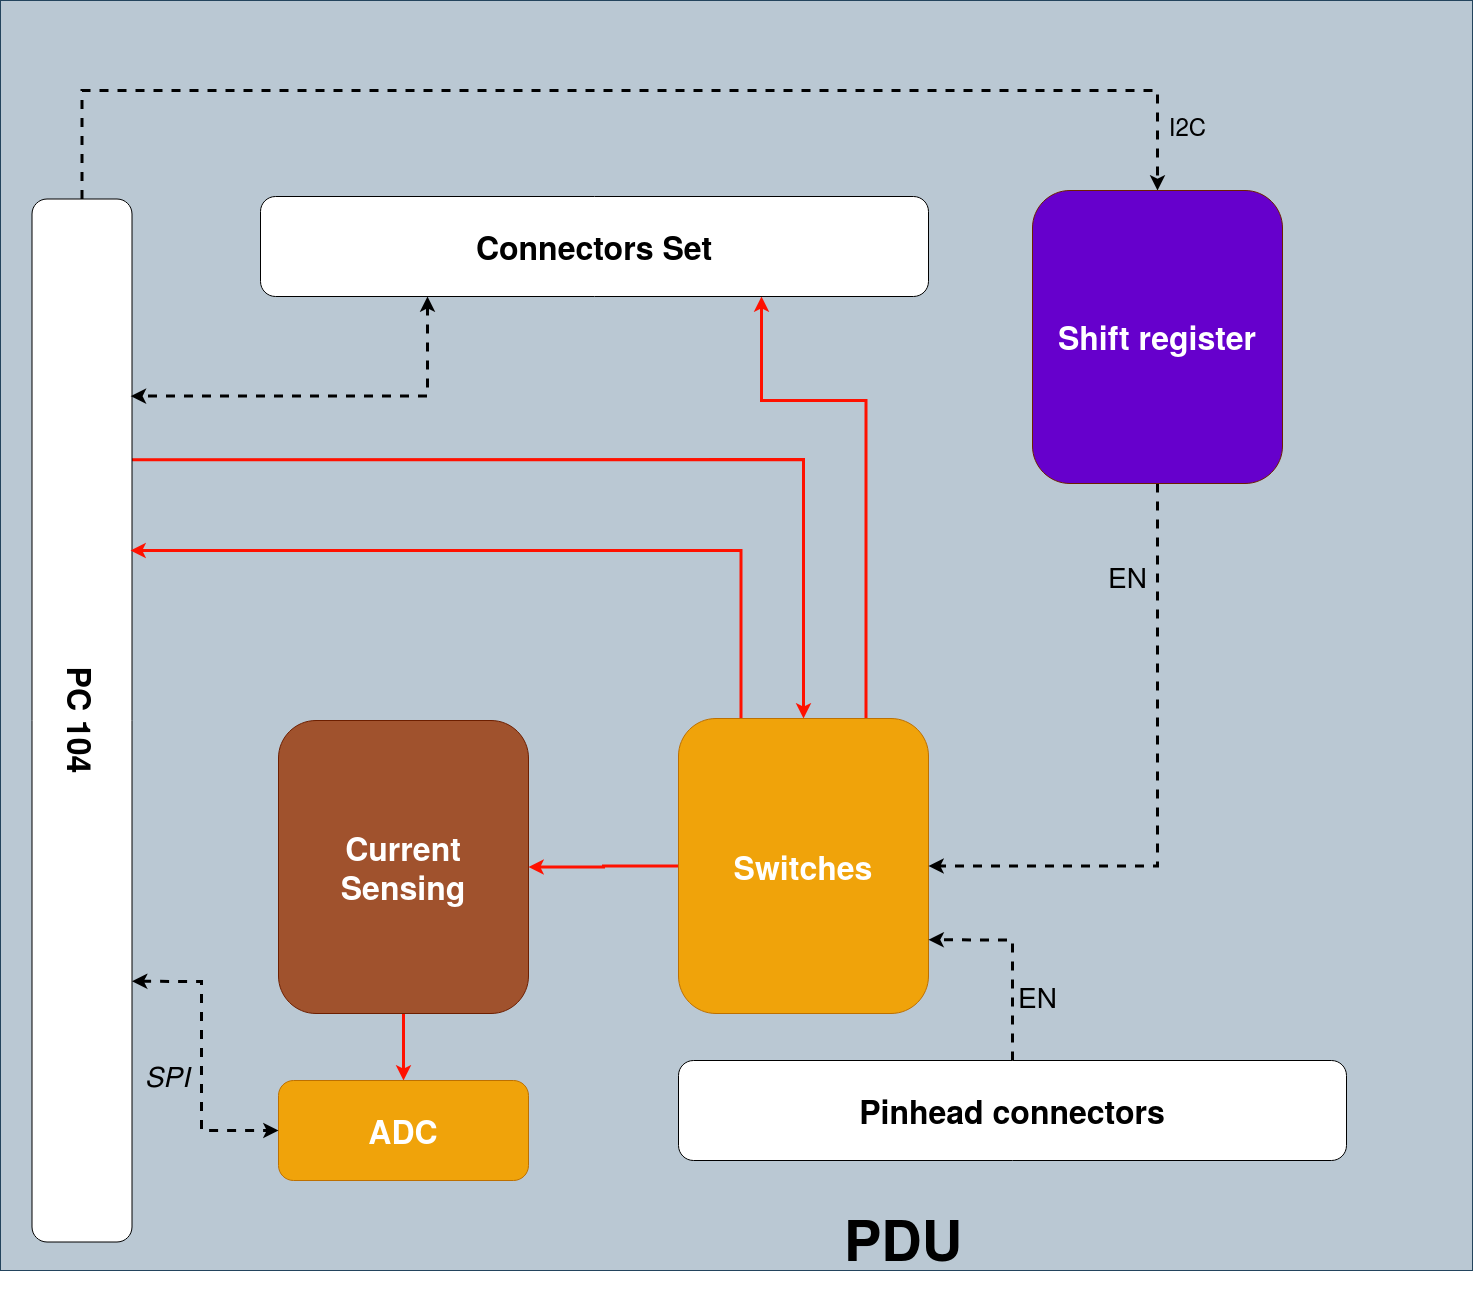
\includegraphics[scale=0.19]{PDU.png}
 	\caption{PDU board}
 	\label{fig: PDU}
 \end{figure} 

\section{Load Switches}
PDU has 23 power load switches which provide commutation of the power lines. In order to fulfill the demanded requirements from Chapter \ref{cha:chapter3}, three types of load switches were chosen: TPS203x, TPS1H200A and FPF2701. 

Tab. \ref{Tab:sw} illustrates the chosen load switches and relative power lines of the PDU.
\captionof{table}{Switches and power lines of the PDU}
\begin{tabular}{p{2cm}p{2cm}p{2cm}p{2cm}p{2cm}p{2cm}} \toprule
	Channel & Switch  & Voltage [V] & Type & Output\\ \midrule
	VCC0 & TPS203x & 3.3, 5 & BUS & PC104\\
	VCC1 & TPS203x & 3.3, 5 & BUS & PC104\\
	VCC2 & TPS203x & 3.3, 5 & BUS & PC104\\
	VCC3 & TPS203x & 3.3, 5 & BUS & PC104\\
	VCC4 & TPS203x & 3.3, 5 & BUS & PC104\\
    VCC5 & TPS203x & 3.3, 5 & BUS & PC104\\
    VCC6 & TPS1H200A & 5, Vbat & BUS & PC104\\
    VCC7 & TPS1H200A & 5, Vbat & BUS & PC104\\
    VCC8 & TPS203x & 3.3, 5 & Payload & Side con.\\
    VCC9 & TPS203x & 3.3, 5 & Payload & Side con.\\
    VCC10 & TPS1H200A & 5, Vbat & Payload & Side con.\\
    VCC11 & TPS1H200A & 5, Vbat & Payload & Side con.\\
    VCC12 & TPS1H200A & 5, Vbat & Payload & Side con.\\
    VCC13 & TPS1H200A & 5, Vbat & Payload & Side con.\\
    VCC14 & TPS1H200A & 5, Vbat & Payload & Side con.\\
    VCC15 & TPS1H200A & 5, Vbat & Payload & Side con.\\
    VCC16 & TPS203x & 3.3, 5 & Payload & Side con.\\
    VCC17 & TPS203x & 3.3, 5 & Payload & Side con.\\
    VCC18 & TPS1H200A & 5, Vbat & Payload & Side con.\\
    VCC19 & TPS203x & 3.3, 5 & Payload & Side con.\\
    COM0 & FPF2701 & 7.4 & BUS & PC104\\
    COM1 & FPF2701 & 7.4 & BUS & PC104\\
    HISP & TPS1H200A & 5, Vbat & BUS & PC104\\ \\
	\bottomrule
	
\end{tabular}\\ \\ \\ \\
\label{Tab:sw}

Every switch has an ability to determine over current($\overline{OC}$)of its power line and provide a FAULT signal to the microcontroller. After receiving a FAULT signal,  microcontroller toggles the switches with adjusted delay in order to prevent latch up of the power lines. All pins of the $\overline {OC}$ switches are connected using star-type to one pin of the P1 connector, which prevents system destruction due to a single node failure.

In addition, the required current limit of each switch of the PDU board can be adjusted by configuring the resistors value or changing the type of chips that fit to the IC's footprint.   
  \\ \\
\subsection{TPS203x }
The TPS203x switch has an operating voltage of 2.7V to 5.5V, which can be used for both 3.3V and 5V power lines. TPS203x is an easy to use 8 pin micro chip. Fig. \ref{fig: PDU332} illustrates the pinout of the load switch TPS203x.

\begin{figure}[h]
	\centering
	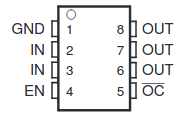
\includegraphics[scale=0.6]{tps203x.png}
	\caption{TPS203x \cite{26}}
	\label{fig: PDU332}
\end{figure} 

TPS203x has two power input pins 2,3 and three output pins 6, 7, 8. Load switch enable control, provided via EN pin 4. TPS203x also has a required ability to provide an over current signal by pin number 5 $\overline{OC}$. \cite{26} When the output load exceeds the current, $\overline{OC}$ getting LOW and the switch limits the output current to a safe level by switching into a constant current mode. TPS203x has 4 different types of chips: TPS2030, TPS2031, TPS2032, TPS2033, TPS2034. All of these chips have a different current threshold. Current limit of five TPS203x types shown on the table \ref{Tab:curr}.\\

\captionof{table}{Types of TPS203x and their curret limits\cite{26}}
\begin{tabular}{p{4cm}p{5cm}p{4cm}} \toprule
	Switch type & Recommended max continuous  current [A] & Current Limit [A]\\ \midrule
	TPS2030 & 0.2 & 0.3\\
	TPS2031 & 0.6 & 0.9\\
	TPS2032 & 1 & 1.5\\
	TPS2033 & 1.5 & 2.2 \\
	TPS2034 & 2 & 3 \\
	
	\bottomrule
	
\end{tabular}\\ \\ \\ \\
\label{Tab:curr}

Each type of TPS203x switch has been selected to meet the requirements of the power line according to Table \ref{Tab:curr}. Switch TPS2030 is used on the lines: VCC0, VCC1, VCC3, VCC4, VCC5, VCC9 and VCC19  where supplied  load current does not exceed the limit of 0.2A. Switch TPS2031 is used on the line VCC17 for the LORA payload where supplied load current does not exceed the limit of 0.6A. Switch TPS2032 is used on the line VCC8 for the AURA payload where load current does not exceed the limit of 1A. Switch TPS2033 is used on the line VCC2 for the ADCS where supplied load current does not exceed the limit of 1.5A. Switch TPS2034 is used on the line VCC16 for the antenna release mechanism where supplied load current does not exceed the limit of 3A. \\

Figure \ref{fig: vcc0} illustrates the switch TPS2030 on the power line VCC0, which is used to supply power to the OBC.

\begin{figure}[h]
	\centering
	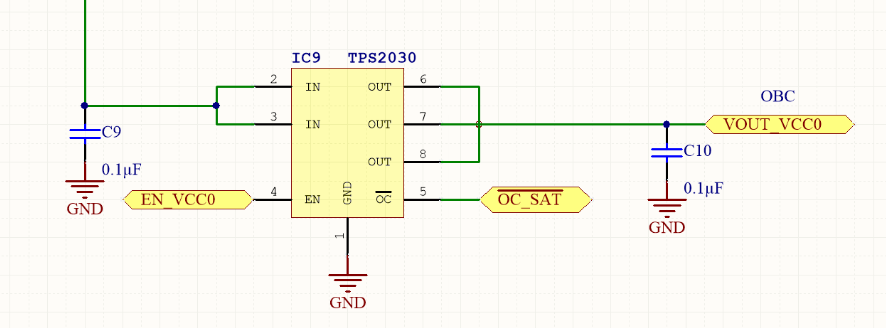
\includegraphics[scale=0.4]{tps203x_.png}
	\caption{TPS2030 on the VCC0 channel}
	\label{fig: vcc0}
\end{figure} 

On the Fig. \ref{fig: vcc0}, two bypass capacitors C9 and C10 used to filter the signal and to improve the immunity of the device to short-circuit transients.   Additionally, 10k pull up resistor connected to the $\overline{OC}$ (10K pull up resistor shown in Appendix B). \\ \\

\subsection{FPF2701}

FPF2701 has an operating voltage 2.8 to 36V and 0.4 to 2A adjustable current limit. FPF2701 has an SO8 footprint package. In addition, FPF27001 was used on previous 3U satellite missions.\\

Fig. \ref{fig: fpf2712} illlustrates the pinout of the FPF2701 load switch.

\begin{figure}[h]
	\centering
	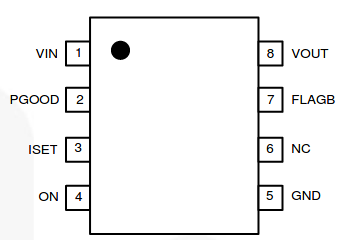
\includegraphics[scale=0.3]{fpf2701.png}
	\caption{FPF2701 \cite{27}}
	\label{fig: fpf2712}
\end{figure} 

FPF2701 is the 8 pin load switch which is used for the UHF power line commutation. FPF2701 completely fulfill requirements TL13, TL14 from Chapter \ref{cha:chapter3} regarding the UHF power supply. It can handle the required voltage of 7.4V and adjust the current to needed 690mA. The most important feature of FPF2701 load switch is the inverted enable input(active LOW).\\

Pin 1 is a power input pin which can handle the voltage between 2.8 and 36V. Pin 3 ISET used to adjust the current limit of the load switch. \cite{27} "The  current  limit  ensures  that  the  current  through  the switch  doesn't  exceed  a  maximum  value  while  not limiting  at  less  than  a  minimum  value.  The current-limit level    is    adjustable    through    an    external    resistor connected between the ISET pin and GND. " The formula \ref{eq:fpf} shows the calculation of the resistor value for intended current limit value.

\begin{equation}\label{eq:fpf}
R_{set}(k\Omega) = \frac{277.5}{I_{lim}(A)}
\end{equation}

For the Descartes mission, the current limit $I_{lim}$ was defined to 2A to prevent an inrush current pike influence, which was achieved by setting the resistor to 140K.

Pin 4 of the FPF2701 is an inverted enable pin, which was required according to FR7 the Chapter \ref{cha:chapter3}. FLAGB (pin 7) is an open-drain pin that provides a signal to notify the microcontroller that the set current has been exceeded at pin ISET. FLAGB supplies 3.3 V output to the microcontroller. In case the current limit is exceeded, the control logic of the chip sends signal to the inner MOSFET that connect ground with the pin. All fault pins such as $\overline{OC}$, FLAGB  are connected to the one connector pin with a star type, which prevent the system from collapsing in case of the failure of one node.

Fig. \ref{fig: fpf27_schema} illustrates the 

\begin{figure}[h]
	\centering
	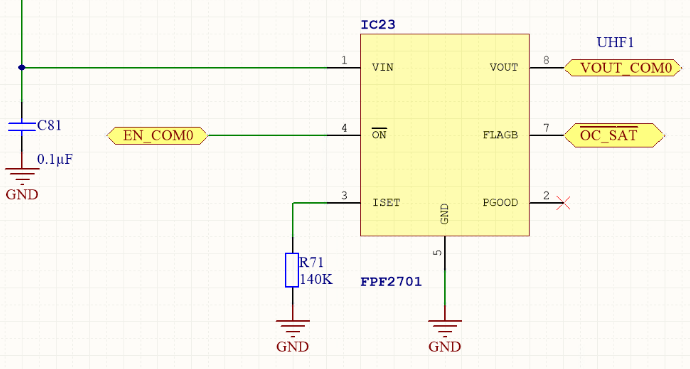
\includegraphics[scale=0.3]{fpf2701_pic.png}
	\caption{FPF2701 on the COM0 power line}
	\label{fig: fpf27_schema}
\end{figure} 

\subsection{TPS1H200A}

TPS1H200A has an operating voltage 3.4V to 40V and an adjustable current up to 6A. TPS1H200A has a 8-pin HVSSOP footprint package. Descartes Mission and PDU design, according to top level requirements, TL1 and TL3, require a switch capable of switching the voltage of 5V and 7.4V which is inside the tolerance of the TPS1H200A chip. The second reason for choosing the TPS1H200A chip is the ability to set the current limit with an external regulating resistor that meets the FR5 requirement. The third reason is the ability to detect line overload and notify the microcontroller. Moreover, the chip was used for previous satellite missions \cite{28}.\\

Descartes Mission requires eight Vbat power lines, where Vbat equals 7.4V. However, PDU design consists of ten power lines which used TPS1H200A switch. One of the reasons for this is the ability to work at 5V and withstand heavy loads up to 6A. \\ 

Switch TPS1H200A is used for on lines VCC10, VCC11, VCC12, VCC13, VCC14, VCC15 which are used to supply power to DeCor payloads. Also switch TPS1H200A is used on empty lines VCC6, VCC7 and VCC18. Finally, TPS1H200A is used on HISP power line, which provide power to Hispico transceiver. 

TPS1H200A has 8 pins and thermal pad which is connected to GND. Pin 1 is enable pin which activates the power transmission of the switch. Signal to enable pin comes from the GPIO pin of the microcontroller. Pin 2 enables diagnostic function of the TPS1H200A chip. While diagnostic function is activated, TPS1H200A is able to set up current limit, adjust delay and provide a current limit signal to the microcontroller. Pin 3 provides an output signal to the microcontroller when current limit was surpassed. Pin 4 allows to adjust current limit. Current limit threshold can be set by placing an external resistor. Equation \ref{eq: res} shows the resistor value calculation.

\begin{equation}\label{eq: res}
R = \frac{0.8 \times 2500}{I}
\end{equation}


Pin 5 is a DELAY pin which configures the behavior of the chip while over current. When current limit is reached, TPS1H200A supports 3 modes: holding, latch-off and auto retry. For most of the cases TPS1H200A is configured as a latch-off. \cite{28} "When hitting a current limit,the output current holds at the setting current,but latches off after a preset DELAY time ($t_{dl1}$+ $t_{dl2}$). $t_{dl1}$ is the default delay time,and $t_{dl2}$ is a capacitor-configurable delay time." To adjust TPS1H200A as a latch-off external capacitor has to be placed. 

\begin{figure}[h]
	\centering
	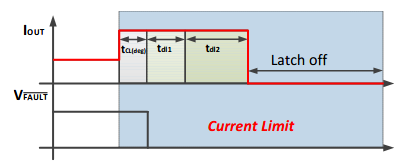
\includegraphics[scale=0.5]{tpscl.png}
	\caption{Latch-off mode\cite{28}}
	\label{fig: tpscl}
\end{figure} 

The time $t_{dl2}$ can be configured by placing an external capacitor. The calculation of $C_{delay}$ is shown in equation \ref{eq: t2}.  \\

\begin{equation} \label{eq: t2}
C_{delay} = \frac{4.5\mu A \times t_{dl2}}{1.45V} 
\end{equation}



 HISP power line, which is needed to supply power to S-band transceiver Hispico, required 5V and load of 1.5A, during the first 0.001s of inclusion Inrush current of the Hispico may reach 4A. The typical inrush current distribution is shown in Figure \ref{fig: hisp_inr}.

\begin{figure}[h]
	\centering
	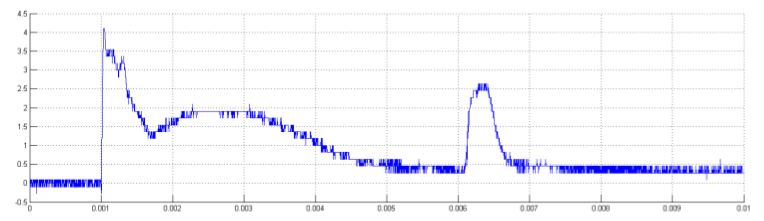
\includegraphics[scale=0.5]{hisp_diag.png}
	\caption{Typical inrush current at startup (0.001 s) in A over time in s}
	\label{fig: hisp_inr}
\end{figure} 

To prevent a critical voltage drop while inrush current, two capacitors with value of 22µF in parallel were placed at output of the load switch. This is illustrated on the figure \ref{fig: hispico}. The value of capacitors was calculated by using formula \ref{eq:3}.

For the TPS1H200A on the HISP channel CL pin is adjusted to 2A and DELAY pin is configured as holding mode. In holding mode \cite{28}"when hitting a current limit,the output current holds at the setting current." This combination was made in order to prevent switch from shutting down while 4A inrush current during the inclusion of Hispico S-band transceiver and keep the threshold at 2A for the required 1.5A load of s-band transceiver. 
 


\begin{figure}[h]
	\centering
	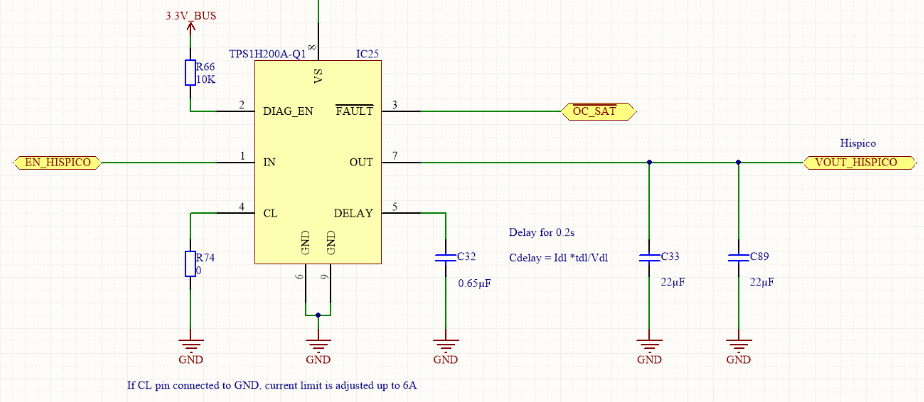
\includegraphics[scale=0.5]{Hispy.png}
	\caption{TPS1H200A on the HISP power line}
	\label{fig: hispico}
\end{figure}



 
\section{Shift Register}\label{shiftty}

Due to the lack of free GPIO pins on the microcontroller, the EPS can only provide 17 GPIO channels for the PDU. Based on this, it was decided to include a shift register into design of the PDU. In the design of the PDU,there are 5 empty power lines VCC4, VCC5, VCC6, VCC7, VCC18 which are not going to be used for Descartes Mission. All this power lines are enabled via shift register as well as VCC19 which is responsible for triggering the power line, that supplies power to the thermo-sensors. The design idea of having empty power channels and thermo-sensors channel on the shift register, is to include less important power lines under shift register control, thereby reducing the risk of pin control via additional device. 


 MAX7328 is a two wire  serial-interfaced peripherals with eight I/O ports and has a 16 pin SO wide footprint package. MAX7328 is general-purpose port expanders operating from a 2.5V to 5.5V supply that provide eight open-drain output ports with a 20mA sink capability. In addition, integrated pull up resistors are used for the I$^2$C line, which are not shown on the Fig. \ref{fig: sr1}.       MAX7328 has a 3 address inputs A0, A1 and A2. Those address inputs can be configured by soldering the external zero ohm resistors to the appropriate input pins \cite{29}.  


\begin{figure}[h]
	\centering
	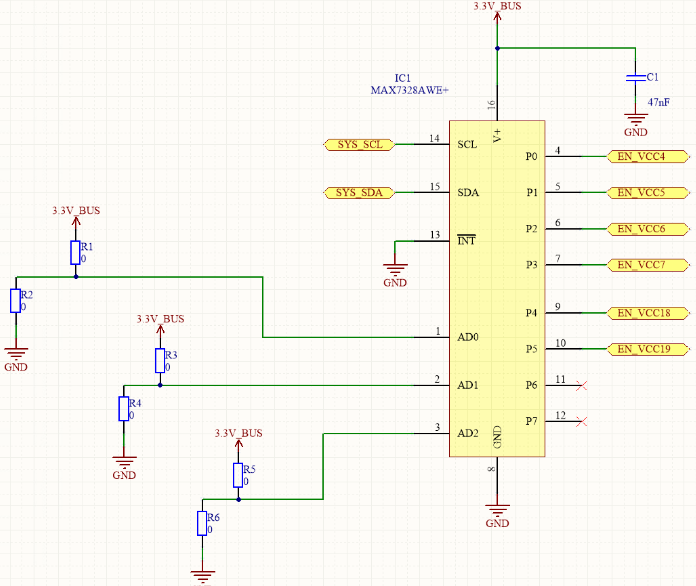
\includegraphics[scale=0.3]{sr.png}
	\caption{ Schematics of the shift register MAX7328}
	\label{fig: sr1}
\end{figure}

The MAX7328 shift register has an easy operation principle. The control of the shift register is implemented via I$^2$C protocol. The microcontroller must communicate with the slave device (MAX7328) by sending the address of the slave device to the I$^2$C bus, which must be accompanied by a confirmation bit. Then the port data can be sent to enable or disable the port. The operation principle of MAX7328 is shown on the Fig. \ref{fig: sr_op1}. 
\newpage
\begin{figure}[h]
	\centering
	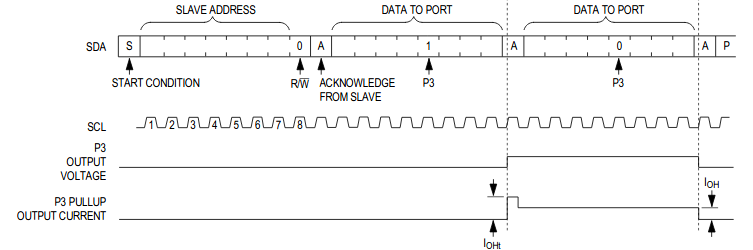
\includegraphics[scale=0.5]{sr_op.png}
	\caption{ MAX7328 operation principle\cite{29}}
	\label{fig: sr_op1}
\end{figure}
 
\section{Current Measurement and Conversion}

Due to the fact that the PDU needs to have 23 current sensors for each power line, it was decided to use 23 analog current sensors in combination with an ADC instead. The main reason for this choice is to keep the flight heritage which was used for previous missions. Secondly is due to the relatively huge amount of sensors on the board. Current sensors that give an output directly to I$^2$C or SPI have a limited amount of slaves which make them unsuitable to use for the current application.\\

For the Descartes mission, the MAX4372T current sensor is used. MAX4372 is a current-sense amplifier which offers a gain of 20. MAX4372T operates on 3.3V and draws 30 µA. MAX4372 has a compact SOT23-5 package with 5 pins. Fig. \ref{fig: max4372t_inside} illustrates the functionality of max4372T current sensor.

 \begin{figure}[h]
 	\centering
 	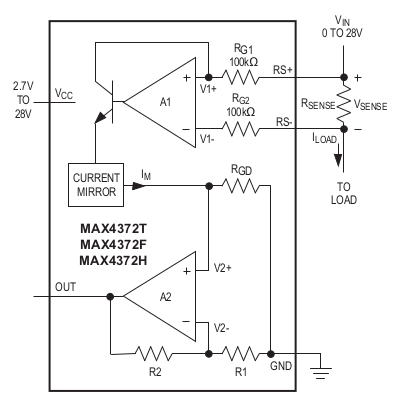
\includegraphics[scale=0.4]{max4372inside.png}
 	\caption{MAX4372T \cite{24}}
 	\label{fig: max4372t_inside}
 \end{figure} 
 
 \newpage
 

 Current flows through the sense resistor, generating a sense voltage.  Since A1’s inverting input is high impedance, the voltage on the negative terminal equals V IN - V SENSE \cite{23}. A1 forces its
positive terminal to match its negative terminal; therefore, the voltage across $R_{G1}\times (V_{IN} - V_{1}-)$ equals $V_{SENSE}$ . This
creates a current flow through $R_{G1}$ equal to $V_{SENSE}$ /
$R_{G1}$ . The transistor and current mirror amplify the current
by a factor of $\beta$. This makes the current flowing out of the
current mirror equal to: 

 \begin{equation}
I_{M} = \frac{\beta \times V_{sense}}{R_{G1}}
 \end{equation}
 A2’s positive terminal presents high impedance, so this
 current flows through $R_{GD}$ , with the following result:
  \begin{equation}
V_{2+} = \frac{R_{GD} \times \beta \times V_{sense}}{R_{G1}}
  \end{equation}
  R1 and R2 set the closed-loop gain for A2, which ampli-
  fies $V_{2+}$, yielding:
  \begin{equation}
  V_{out} = \frac{R_{GD} \times \beta \times V_{sense}}{R_{G1} \times (1+\frac{R2}{R1})	 }
  \end{equation}
The gain of the device equals:
  \begin{equation}
  GAIN =\frac{V_{out}}{V_{sense}} = \frac{R_{GD} \times \beta (1+\frac{R2}{R1})}{R_{G1}}
  \end{equation}
  
  MAX4372 has 3 types of current sensors, for a MAX4372T type, amplification factor equal 20.
  
  Considering different current lines and the fact that ADC has a limited tolerance of the analog input, $R_{sense}$ have to be chosen correctly according to the requirements. According to the datasheet of the ADC(MAX1231) the analog input has to be between $ -0.3V$ and $(V_{DD} + 0.3V)$ where $V_{DD}$ equals 3.3V.
  
  The value of $R_{sense}$ could be calculated with a formula:
    \begin{equation}
    R_{sense} = \frac{V_{out}}{GAIN \times I}
    \end{equation}
  
  Where:\\
  I is a current on the power line\\
  V$_{out}$ is an output voltage\\ 
 
 The Tab. \ref{Tab:res} provides calculated values of the shunt resistors according to the current recuirements of the power lines. V$_{out}$ = 0.5V was chosen as a reference output voltage for the shunt resistor selection. This value is in the tolerance and allows to choose shunt resistor with lower value in order to decrease the voltage drop.
  \newpage
  
  \captionof{table}{Shunt resistor choosing}
   \begin{tabular}{p{3cm}p{3cm}p{2cm}p{2cm}p{3cm}} \toprule
   	Power channel & Load & I$_{max}$ [mA] & V$_{out}$ [V] & R$_{sense}$ [Ohm]\\ \midrule
   VCC0 & OBC & 140 & 0.5 & 0.1\\
   VCC1 & OBC PH & 140 & 0.5 & 0.1\\
   VCC2 & ADCS & 460 & 0.5 & 0.05\\
   VCC3 & ADCS log & 0.06 & 0.5 & 0.5\\
   VCC4 & OBC 5V & 90 & 0.5 & 0.1\\
   VCC5 & OBC 5V & 90 & 0.5 & 0.1\\
   VCC6 & empty & empty & empty & empty\\
   VCC7 & empty & empty & empty & empty\\
   VCC8 & AURA & 600 & 0.5 & 0.05\\
   VCC9 & AMUR & 40 & 0.5 & 0.5\\
   VCC10 & DeCor11 & 40 & 0.5 & 0.5\\
   VCC11 & DeCor12 & 200 & 0.5 & 0.1\\ 
   VCC12 & DeCor21 & 40 & 0.5 & 0.5\\ 
   VCC13 & DeCor22 & 200 & 0.5 & 0.1\\ 
   VCC14 & DeCor31 & 40 & 0.5 & 0.5\\ 
   VCC15 & DeCor32 & 200 & 0.5 & 0.1\\ 
   VCC16 & ARM & 2000 & 0.5 & 0.01\\
   VCC17 & LORA & 200 &  0.5 & 0.1\\
   VCC18 & empty & empty & empty & empty\\
   VCC19 & Term. sens. & 10 & 0.5 & 2.5\\
   COM0 & UHF1 & 690 & 0.5 & 0.05\\
   COM1 & UHF2 & 690 & 0.5 & 0.05\\
   	HISP & HISPICO & 1500 & 0.5& 0.01\\ 
    \bottomrule
   	
   \end{tabular}\\ \\ \\ \\
  \label{Tab:res}
 Another important aspect to consider is the resistance of the power line. The resistance of the power line should be as low as possible to avoid a voltage drop in the presence of high current. In the system design stage, voltage drop can be avoided by providing a low shunt resistor value. In accordance with current requirements, the HISP and VCC16 power channels must provide $ \ geq $ 1500mA, with a resistance of 1Ohm the system will have a voltage drop of $ \ geq $ 1.5V, which will significantly affect the functionality of the output connected device.
 For this reason resistor values for HISPICO and ARM(antenna release mechanism) were chosen with minimal resistance.\\ \\ 
 
 the 6U satellite contains 23 analog outputs from the current sensors which have to be converted into a digital signals. To fulfill this requirement, two analog-to-digital converters MAX1231 are used. MAX1231 has already been used for a previous 3U mission, in order to preserve flight heritage, it was decided to keep this component for the 6U satellite.
 
  MAX1231 is a serial 12 bit  analog-to-digital converter with an internal reference and maximum sampling rate of 300ksps . MAX1231 has a 24 pin configuration with 15 available analog inputs. The device operates at 3.3 V and contains 10 MHz SPI protocol for communication \cite{25}.
  
   \begin{figure}[h]
   	\centering
   	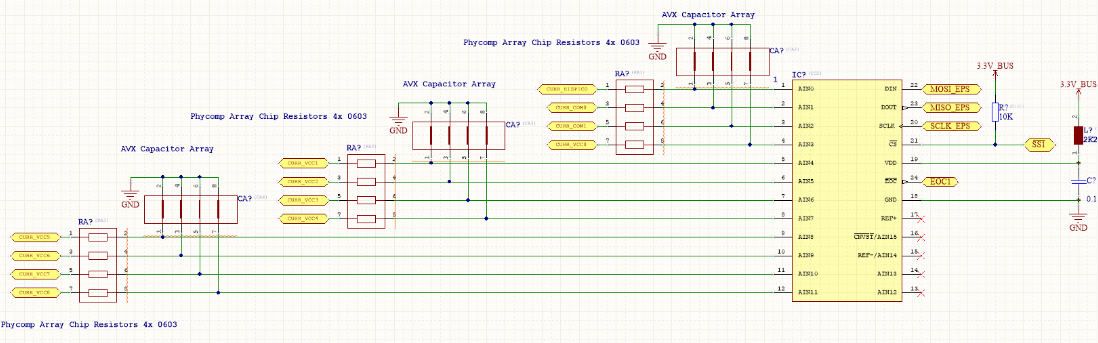
\includegraphics[scale=0.4]{ADC.png}
   	\caption{MAX1231 for Descartes application}
   	\label{fig: adc}
   \end{figure} 
 
  Figure \ref{fig: adc} illustrates the MAX1231 for the Descartes application. This figure shows external connections of the ADC chip. Pins 1 to 12 are used for the analog inputs. Each analog input has a 1k resistor, which is used to protect the ADC and prevent high current input from the sensor. In addition, decoupling capacitors with a capacity of 0.01µF are located in parallel, which are used to filter the input signal. Pins 22, 23, 20 and 21 are used for the SPI communication where pin 21 is a slave select. Pin 24 is the $\overline{EOC}$ End of Conversion output pin used to notify the microcontroller about the end of the conversion. Pin 19 is a power supply pin for the ADC chip, supplied with a 3.3V. To minimize the noise effect, the VDD input bypasses the 0.1 µF capacitor to GND. In addition, 2.2K ferrit chip is connected in series with the supply to improve power-supply filtering. 
  
  
 
  \begin{figure}[h]
  	\centering
  	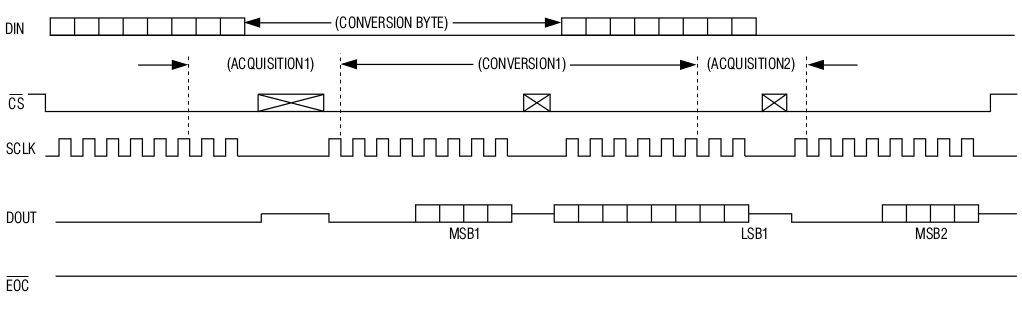
\includegraphics[scale=0.4]{ADC_clock.png}
  	\caption{operation principle of the MAX1231 \cite{25}}
  	\label{fig: adc}
  \end{figure} 
 
 Fig. \ref{fig: adc} illustrates the operation principle of the MAX1231. The MAX1231 has 4 different clock modes. However, the Descartes Mission uses an external clock mode from the microcontroller. To begin communication with the MAX1231, chip select pin has to be latched up in order to define the slave. Then microcontroller sends a conversion register address with the channel information. After the Register address transmission, the slave will send 12 bytes of data separated in two bytes. First receiving byte contains first 4 empty bits which have to be ignored and following 4 bits are the MSB. The second following byte contain the left 8 bits. After the second byte has been sent to the microcontroller, the $ \overline {EOC} $ pin gets HIGH to notify the microcontroller that the conversion is complete, and the $ \overline {CS} $ pin becomes LOW.
 
 \section{Isolators}
 
The operation principle of the electrical isolators is the partial separation of electricity from the system for safety reasons during maintenance work. PDU includes two payload connectors that carry I$^2$C and SPI signals from the payloads. Due to the functional requirement FR4 from chapter \ref{eq:3} every payload I$^2$C and SPI nodes shall have the isolation. For that reason the decision was made to include two types of isolators from previous missions :\\ \\

$\bullet$ ADUM1250\\
$\bullet$ MAX1485\\ \\

ADUM1250 is a hot swappable digital isolators with a bidirectional I2C communication channels. "This eliminates the need to separate I2C signals into separate transmit and receive signals for use with stand-alone optocouplers." Fig. \ref{fig: adum} illustrates the schematics of the ADUM1250 isolator, which isolates the main I$^2$C data line from the payload I$^2$C data line \cite{30}.

 \begin{figure}[h]
 	\centering
 	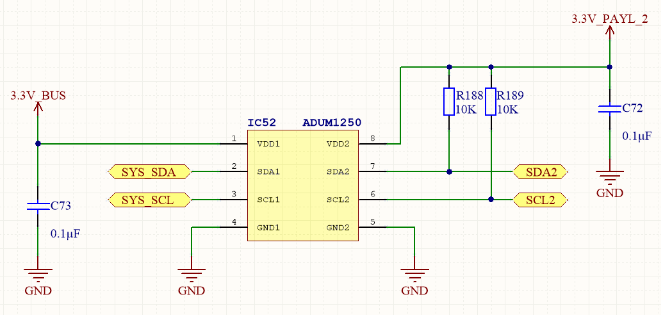
\includegraphics[scale=0.4]{ADUM1250.png}
 	\caption{ADUM1250 isolating main I$^2$C data line from the (payload 2) I$^2$C data line }
 	\label{fig: adum}
 \end{figure} 

 The MAX14850 is a six-channel digital isolator that provides low-cost digital signal transfer between circuits with different power supplies. The MAX14850 provides low power consumption and stable operation at high temperatures. The MAX14850 can be used to insulate SPI buses, I2C buses, RS-232, RS-485 / RS-422 buses, and general purpose insulation. Fig. \ref{fig: adum122} illustrates the MAX14850 isolator which isolates the main SPI from the SPI of the payload \cite{31}.

\begin{figure}[h]
	\centering
	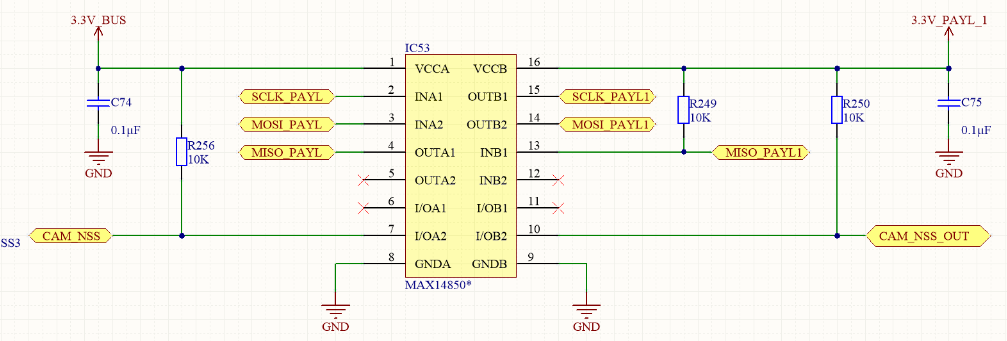
\includegraphics[scale=0.4]{max14850.png}
	\caption{MAX14850 isolating main SPI data line from the (payload 1) SPI data line }
	\label{fig: adum122}
\end{figure} 

\section{Connectors Design}

Power Distribution Unit has 12 connectors on it's design. \\

$\bullet$ Eight payload connectors\\
$\bullet$ Two EPS connectors\\
$\bullet$ One EGSE connector\\
$\bullet$ One PC104 connector\\

PC104 is a main connector which are used to bridge main pcb boards such as the PPU, PDU, OBC, OBC-PH, UHF module and Hispico transceiver.
EGSE connector is used to program the EPS and the OBC microcontrollers, that located on the PPU and the OBC boards.

The EPS connectors P1 and P2 were added into design due to the lack of free pins on the PC104 connector. These connectors are used to transfer the data signals and power pines between the PPU and the PDU. The EPS connectors provide an enable signals from the EPS microcontroller directly to the PDU via P2 connector and bus power lines 3.3V and 5V via P1 connector.

  \begin{figure}[h]
  	\centering
  	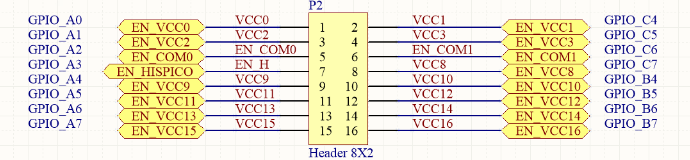
\includegraphics[scale=0.4]{EPSCON.png}
  	\caption{EPS connector P2}
  	\label{fig: EPSCON}
  \end{figure} 

Payload connectors have a primary function to transfer the signals and power to the payload. Eight payload connectors are divided into 8-pin connectors and 9-pin connectors. 8-pin connectors are designed to carry payloads that require UART and CAN protocols. The 9th pin is required for the payloads that transfer I$^2$C and SPI protocols in order to give a power feedback into the ADUM1250 or MAX14850 isolators.  

Two payload connectors, K10 and K11 were included for the possible opportunity to handle a payload that require a I$^2$C or SPI protocols.
The connection design of the connector K10 is illustrated on the figure \ref{fig: iso1}. To adjust the signal input between I$^2$C and SPI simple zero ohm resistors are used.

\begin{figure}[h]
	\centering
	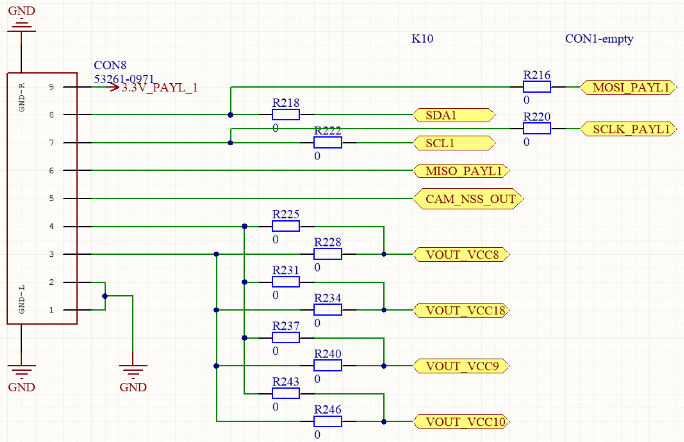
\includegraphics[scale=0.4]{iso1.png}
	\caption{Payload connector K10}
	\label{fig: iso1}
\end{figure} 
 
The PDU is designed in such a way that all payload connectors have an opportunity to be supplied from different power sources and with different voltages. The reason for this is because of the functional requirement, FR1 in chapter \ref{eq:3}. This design allows the PDU to be compatible with every payload requirement. Each payload connector has the ability to transfer at least 3.3V, 5V and 7.4V to the payload.  This requirement was accomplished with a zero ohm  resistors  design which can configure the input of the power supply to the payload connector.\\

All of the connectors and their pin descriptions are shown in Appendix A. 

 
  
  
    \chapter{PCB realization\label{cha:chapter5}}

The PCB of PDU was designed and realized. All PCB work from schematics to net list wiring board layout design and finally post processing, was done via Computer Assisted Design Altium Designer. 

\begin{figure}[h]
	\centering
	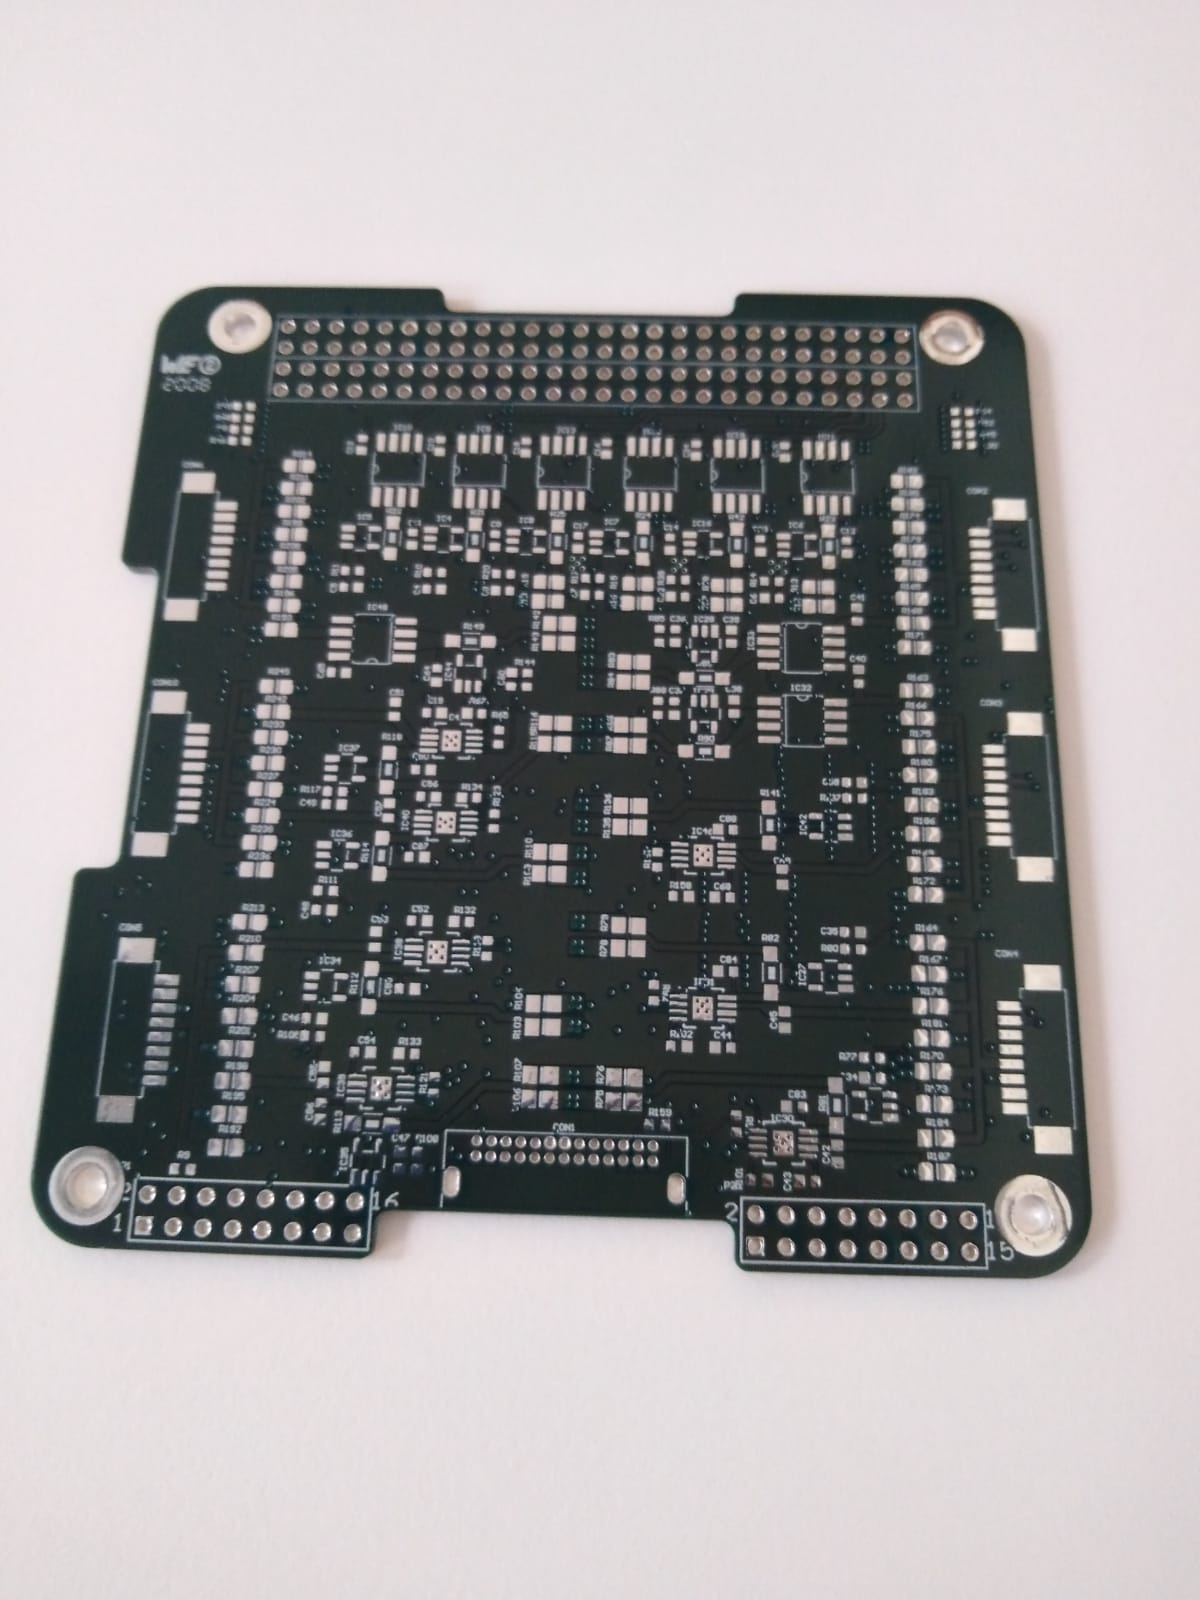
\includegraphics[scale=0.2]{PDU_PCB.jpeg}
	\caption{Power Distribution Board PCB}
	\label{fig: PCB_PDU}
\end{figure} 

\section{Physical Dimensions}

PCB design rules such as board dimensions, max trace width, component-to-component distance, max vias size pad-to-pad distance are all contained within the German Orbital Systems templates and requirements, as well as the manufacturer requirements. 

The total thickness of the PCB is 1.7 mm. The PCB of the PDU has eight copper layers with 0.036 mm each. Every copper layer separated with dielectric material FR-4 with thickness of 0.254 mm. FR-4 is a typical composite material composed of woven fiberglass with epoxy resin binder. 


\begin{figure}[h]
	\centering
	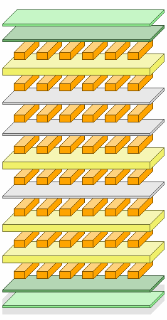
\includegraphics[scale=0.8]{layer1.png}
	\caption{Layer stack}
	\label{fig: layerstack}
\end{figure} 


The required PDU dimensions for the length and width are 90.16mm x 95.90mm. These dimensions are standardized by German Orbital Systems.

\section{Layout design}

The layout design was started with the power trace width calculation.
According to the power requirements, maximum supplied current of the on the PDU for the Descartes mission is 1.5A which has to be supplied to Hispico S-band transceiver. The minimal width of the power lines on the PDU is not less than 0.8 mm.

The maximum current can be calculated by equation \ref{eq: amp}

\begin{equation}\label{eq: amp}
I = K \times dT^{0.44} \times (W \times H)^{0.725}
\end{equation}

Where\\

I - Max current\\
K - Coefficient for external traces (0.048)\\
W - Width in mils(0.8)\\
H - Thickness in mils(0.036) \\
dT - Temperature rise above ambient in $^\circ$C(10)\\

As a result, maximum current that can be transfered through the track is 2.07631 $\approx$ 2A.\\ 

Power Distribution Unit PCB has eight copper layers. Top and bottom layers used for power transmission, partially as a signal transmission and as a ground polygon. Second and the seventh layers used for a signal transmission. The design of the second and seventh layers is designed so that the signal lines having a track width of 0.4 mm are as straight as possible to reduce noise. The third and sixth layers are ground layers they are used for decoupling the signal layers as well as for a thermal dissipation reasons, which is an important function considering the fact that PDU  transfer power. Fourth and fifth layers are power layers, they consist of the power polygons which transfer power from the source to the integrated chips and to the connectors.   

\begin{figure}[h]
	\centering
	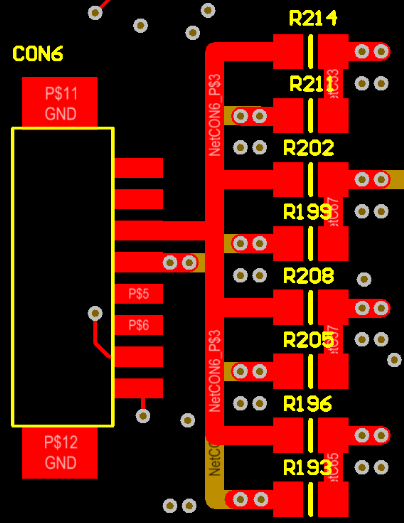
\includegraphics[scale=0.4]{resist_con.png}
	\caption{Zero ohm resistors to payload connector network}
	\label{fig: res}
\end{figure} 


Figure \ref{fig: res} shows only top, middle power layers and top silk overlay of the PCB.

  
The main feature of the Power Distribution Board layout design is a flexibility of a choice of a connector, power line and required voltage. PDU has an ability to set up the connector with the different switch power outputs. PDU as it was explained in the chapter \ref{sec:tech77} used two types of connectors 9-pin connector and 8-pin connector. Each of those two types has a two input power pins for a power transmission.  Some connectors in the Descartes mission required 2 inputs from two different switches such as connectors: K5, K6, K7 which have to transfer power to the DeCor payload. The connector designations are given in Appendix. The zero ohm resistors allows to select the power channels that will supply power to the payload connector, and then to the payload. Each payload connectors can be adjusted to receive power from one of the four load switches. Figure \ref{fig: res} shows example of the connection layout design between zero ohm resistors and the payload connector. Zero ohm resistors placed maximum close to the payload connector in order to make more space on the PCB. All zero ohm resistors that used for a power transfer are 0805 inch due to the high power.

The load switches are located on the top and bottom side of the PCB. Each switch must supply power to a specific connector in order to reduce the length of the power path between the switch and  corresponding connector, the switches were located as close to their respective connectors as possible to reduce path loss and resistance, which directly affects the voltage drop. 

\begin{figure}[h]
	\centering
	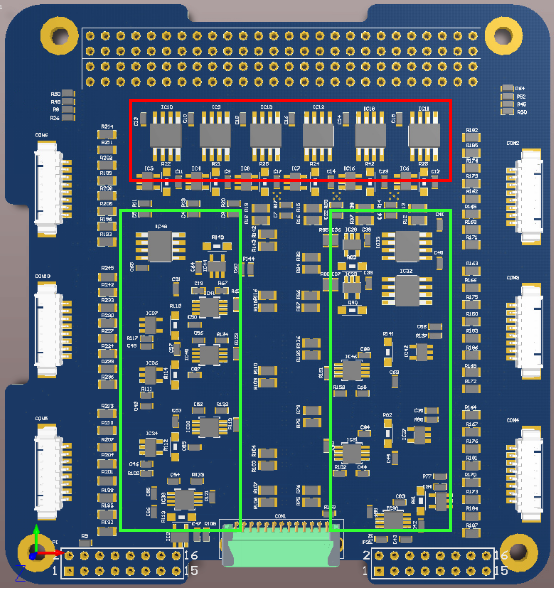
\includegraphics[scale=0.5]{pdu_top_3d_new.png}
	\caption{Top view of the PDU}
	\label{fig: toppducon}
\end{figure} 

Figure \ref{fig: toppducon} shows a the placement of the switches on the top layer of the PDU. Switches, responsible for a bus power line commutation are emphasized with a red frame. In order to decrease the distance between the load switches and PC104 connector, which is used to transfer bus power to oder boards in the stack, switches were located on the top side of the the PCB in the row. The payload switches, that emphasized with green frames, located on the left and right sides of the PCB. This allow them to transfer power without extra losses on the shortest distance to the relative payload connectors.

\begin{figure}[h]
	\centering
	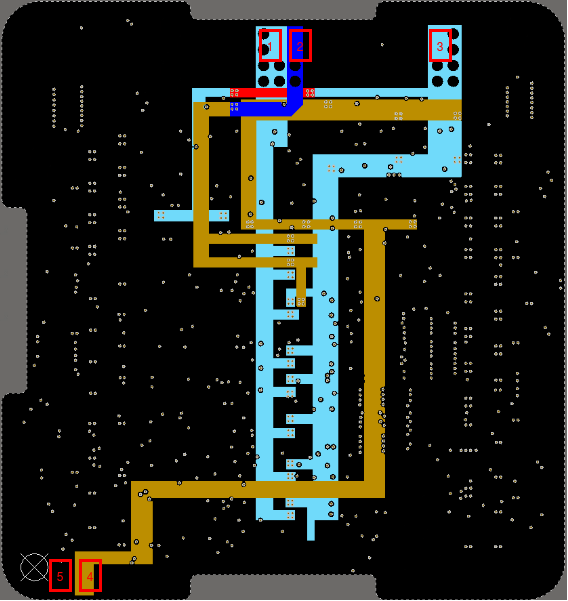
\includegraphics[scale=0.5]{polygons.png}
	\caption{Power polygons of the PDU}
	\label{fig: poly}
\end{figure} 

Fourth and fifth copper layers of the PCB used to transfer a high power. One of the main tasks of the middle power layers is to transfer current from the source pads to the relative IC via polygons. There are 5 main power source pads on the PCB: 7.4V, 3.3V BUS, 3.3V PAYL, 5V BUS, 5V PAYL. Figure \ref{fig: poly} illustrates the main power sources on the PCB, where:\\ \\
 1 - 5V PAYL\\
 2 - 3.3V PAYL\\
 3 - 7.4V\\
 4 - 5V BUS\\
 5  - 3.3V BUS\\

The minimum width of the polygons was calculated according to the formula \ref{eq: amp} and the maximum current with the coefficient of internal traces.

\begin{equation}
W = \frac{\sqrt[0.725]{\frac{1.5}{0.024 \times 10^{0.44}}}}{0.036}
\end{equation} 

According to the upper mention calculation, minimal required inner width of the trace should be not smaller then 1.36 mm. The minimal width of the Power distribution board inner traces is 1.5 mm which within the required tolerance. 



\begin{figure}[h]
	\centering
	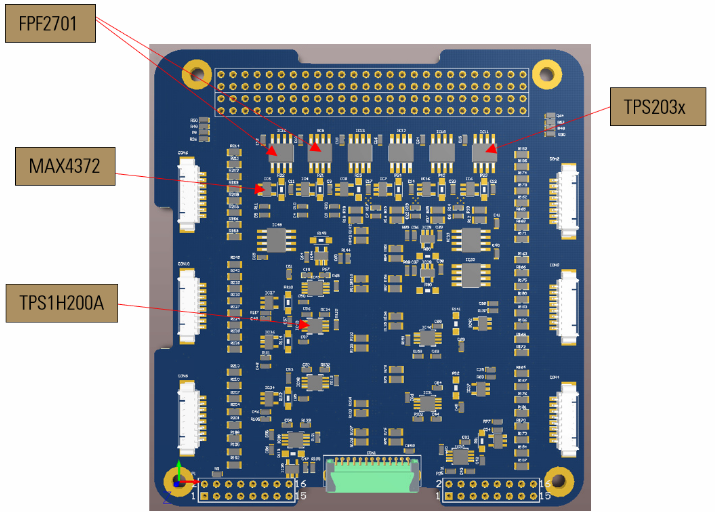
\includegraphics[scale=0.38]{pdu_top_component.png}
	\caption{Types of components on  top view of the PDU }
	\label{fig: pdu_comp_top}
\end{figure} 

\begin{figure}[h]
	\centering
	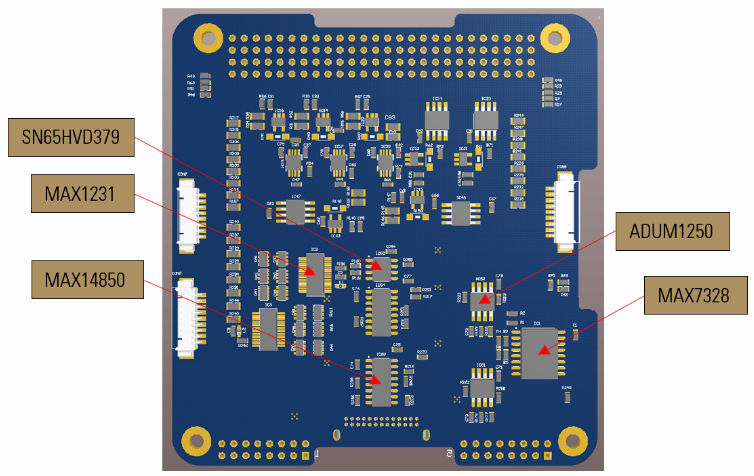
\includegraphics[scale=0.38]{pdu_bot_component.png}
	\caption{Types of components on  bottom view of the PDU}
	\label{fig: pdu_comp_bot}
\end{figure} 


Figures \ref{fig: pdu_comp_top} and \ref{fig: pdu_comp_bot} show placement of components on the PCB.
 



    \chapter{Evaluation\label{cha:chapter6}}

In this chapter the implementation of Component X is evaluated. An example instance was created for every service. The following chapter validates the component implemented in the previous chapter against the requirements.
\\
\\
Put some screenshots in this section! Map the requirements with your proposed solution. Compare it with related work. Why is your solution better than a concurrent approach from another organization?

\section{Test Environment\label{sec:testenvir}}

Fraunhofer Institute FOKUS' Open IMS Playground was used as a test environment for the telecommunication services. The IMS Playground ...

\section{Scalability\label{sec:scal}}

Lorem Ipsum

\section{Usability\label{sec:usab}}

Lorem Ipsum

\section{Performance Measurements\label{sec:performance}}

Lorem Ipsum
    \chapter{Conclusion\label{cha:chapter7}}

 \begin{figure}[h]
 	\centering
 	\includegraphics[scale=0.6]{EPS!.png}
 	\caption{EPS assembly (PDU, PPU, Battery board}
 	\label{fig: EPS!}
 \end{figure}

This thesis described the development of the Power Distribution Unit that is designed in combination with Power Processing Unit and Battery case Unit to supply a 6U satellite with  continuous power.\\  


Massive work was made to accomplish all requirements and develop the PDU.
 

 One of the biggest challenges during the PDU design was the switch selection, and their placement on the PCB layout, taking into account the amount of components on the layout and the power channels requirements such as needed voltage, current, the trace width, size and ability to determine an over-current. Another big challenge was the layout structure of the PDU. Due the fact that the PDU should not only be the distribution board for one Descartes Mission, but an universal distribution unit. PDU might be adjusted for different upcoming missions without change of the design, but making little patch such as resistor replacement made master thesis arduous and interesting at the same time. During the tests PDU had some issues with a voltage drop on the Hispico line while initiation of S-band transceiver. The voltage drop occurred due to the high inrush current of the Hispico transceiver.    However, after adding an extra capacitors on the output of the switch, voltage drop was reduced and results were satisfactory.    \\

PDU was tested using microcontroller Nucleo STM32L073Rz with PSU as a power source and with an electrical load to simulate the load. 

After successful results, the PDU was tested using flight hardware such as PPU, which included a microcontroller to control the switches and receive data from current sensors, a battery board that provided power for the PDU, and payloads. 

Power Distribution Unit fits comfortably withing the mechanical structure of the 6U satellite, all the connectors are easily accessible. 
\\
The Power Distribution Board was designed by using Altium Designer and fabricated by Würth Electronics GmbH. All components were soldered by hands and tested according to the test procedure, described in the Chapter \ref{6}. Most of the used components have flight heritage from previous missions, which makes the PDU more promising for the upcoming projects.  \\ 
PDU was developed following the standardized design which includes the board dimensions (90.16x95.9mm) and PC104 connector location.
Due to the standardized design, it allows PDU to be implemented for a 1U, 2U and 3U satellites. \\
Although PDU was developed and successfully tested for a Descartes Mission, there is still space for a future contributions and improvements. The first possible improvement would be a placement of a zero ohm resistor in the parallel to the isolator. This improvement will give an opportunity to choose if isolator is needed. The reason for this improvement occurred while the temperature sensors test connected to the K11. Initially K11 connector was designed for a payload. According to the functional requirements FR4, PDU shall have isolation for every payload node. However, for a Descartes mission K11 connector was used for a thermal sensors which are part of the satellite bus and have their own isolation. Although TPS203x switches have a flight heritage, relatively simple and robust, they are bulky and can not be adjusted for a current limit by changing resistance value, which is a sensitive disadvantage which might be changed in the future versions.  \\ \\

In conclusion, Power Distribution Board was successfully designed,  manufactured, tested according to all requirements and ready to fly. 


% ---------------------------------------------------------------
\backmatter % no page numbering from here
    \addchap{List of Acronyms}

\begin{tabbing}
spacespacespace \= space \kill

ADC  \> Analog to Digital Converter\\
ARM \>  Antenna release mechanism\\
EPS \>      Electrical Power System\\
MPPT \>    Maximum Power Point Tracking\\
MSB \>      Most Significant Bit\\
LSB \>      Least Signigicant Bit\\
\end{tabbing}
\endinput

		
		% if you want to provide a glossary with explanations of important terms put it in here

    \bibliographystyle{geralpha}
    \bibliography{./bib/references}
    
    \chapter{Annex}

\begin{appendix}
	\section*{Appendix A}
	
	\caption{Pin configuration of PC104 connector}
	\begin{longtable}{p{3cm}p{6cm}}
		\toprule
		Pin & Description \\ \midrule
		C1-1 & PCU CAN1 Interface L \\ 
		C1-3 & PCU CAN1 Interface H \\ 
		C1-12 & JTDI\_OBC \\ 
		C1-13 & JTCK\_OBC \\ 
		C1-14 & JTMS\_OBC \\ 
		C1-15 & JTDO\_OBC \\ 
		C1-16 & JTRST\_OBC \\ 
		C1-17 & PCU UART1 Interface RX \\ 
		C1-18 & PCU UART1 Interface TX \\ 
		C1-27 & OBC Current Sensor \\ 
		C1-31 & PCU Watchdog Disable Pin \\ 
		C1-32 & EGSE Battery Charge Power Input \\ 
		C1-33 & Output Voltage HISPICO \\ 
		C1-34 & PCU CAN2 Interface L \\ 
		C1-35 & 3.3V PCU EPS JTAG \\ 
		C1-36 & PCU CAN2 Interface H \\
		C1-39 & PCU UART4 Interface TX \\ 
		C1-40 & PCU UART4 Interface RX \\
		C1-41 & PCU I2C Interface SDA \\ 
		C1-43 & PCU I2C Interface SCL \\ 
		C1-45 & Output Voltage 0 \\ 
		C1-46 & Output Voltage 1 \\ 
		C1-47 & Output Voltage 2 \\ 
		C1-48 & Output Voltage 3 \\ 
		C1-49 & Output Voltage 4 \\ 
		C1-50 & Output Voltage 5 \\ 
		C1-51 & Output Voltage 6 \\ 
		C1-52 & Output Voltage 7 \\ 
		C2-9 & PCU UART4 Interface RX \\ 
		C2-10 & PCU UART4 Interface TX \\ 
		C2-11 & Output Voltage COM0 \\ 
		C2-12 & GND \\
		C2-13 & PCU UART4 Interface RX \\ 
		C2-14 & PCU UART4 Interface TX \\ 
		C2-15 & Output Voltage COM1 \\ 
		C2-16 & GND \\ 
		C2-17 & PCU SPI Interface MISO \\ 
		C2-18 & PCU SPI Interface MOSI \\ 
		C2-19 & PCU SPI Interface SCLK \\ 
		C2-20 & JTDI EPS \\ 
		C2-21 & JTCK EPS \\ 
		C2-22 & JTMS EPS \\ 
		C2-23 & JTDO EPS \\ 
		
		C2-24 & JTRST EPS \\ 
		C2-25 & 5V Output Voltage \\ 
		C2-26 & 5V Output Voltage \\ 
		C2-27 & 3.3V Output Voltage \\ 
		C2-28 & 3.3V Output Voltage \\ 
		C2-29 & GND \\ 
		C2-30 & GND \\ 
		C2-31 & AGND \\ 
		C2-32 & GND \\ 
		C2-35 & System Power IN \\ 
		C2-36 & System Power IN \\ 
		C2-41 & Remove-Before-Flight Output \\ 
		C2-42 & Remove-Before-Flight Output \\ 
		C2-44 & PCU Watchdog Disable Pin \\ 
		C2-45 & Battery Voltage Output \\ 
		C2-46 & Battery Voltage Output \\
		C2-50 & Slave select 3 \\
		C2-51 & Slave select 4 \\ 
		\bottomrule
		\end{longtable}
		\label{pc104}
		
		
		
		\caption{Pin configuration of payload  connector K9}
		\begin{center}
			
		
		\begin{tabular}{p{3cm}p{3cm}}
			\toprule
			
			Pin & Description \\ \midrule
			1 & GND \\ 
			2 & GND \\ 
			3 & PWR \\ 
			4 & PWR \\ 
			5 & - \\ 
			6 & - \\ 
			7 & CAN1L \\ 
			8 & CAN1H \\ 
			\bottomrule
		\end{tabular}
		\label{k9}
	\end{center}
	
	
	
		\caption{Pin configuration of payload  connector K7}
		\begin{center}
			
			
			\begin{tabular}{p{3cm}p{5cm}}
				\toprule
				
				Pin & Description \\ \midrule
				1 & GND \\ 
				2 & GND \\ 
				3 & PWR \\ 
				4 & PWR \\ 
			5 & UART2\_RX/UART2\_RX\_B \\ 
			6 & UART2\_TX/UART2\_RX\_A \\ 
			7 & UART2\_TX\_Y / CAN2L \\ 
			8 & UART2\_TX\_Z / CAN2\_H \\ 
				\bottomrule
			\end{tabular}
			\label{k7}
		\end{center}
	
	
		\caption{Pin configuration of payload  connector K6}
		\begin{center}
			
			
			\begin{tabular}{p{3cm}p{3cm}}
				\toprule
				
				Pin & Description \\ \midrule
				1 & GND \\ 
				2 & GND \\ 
				3 & PWR \\ 
				4 & PWR \\ 
				5 & - \\ 
				6 & - \\ 
				7 & CAN1L \\ 
				8 & CAN1H \\ 
				\bottomrule
			\end{tabular}
			\label{k6}
		\end{center}
	
		\caption{Pin configuration of payload  connector K3}
		\begin{center}
			
			
			\begin{tabular}{p{3cm}p{3cm}}
				\toprule
				
				Pin & Description \\ \midrule
				1 & GND \\ 
				2 & GND \\ 
				3 & PWR \\ 
				4 & PWR \\ 
				5 & UART1\_RX \\ 
				6 & UART1\_TX \\ 
				7 & CAN2L \\ 
				8 & CAN2H \\ 
				\bottomrule
			\end{tabular}
			\label{k3}
		\end{center}
	
		\caption{Pin configuration of payload  connector K4}
		\begin{center}
			
			
			\begin{tabular}{p{3cm}p{3cm}}
				\toprule
				
				Pin & Description \\ \midrule
				1 & GND \\ 
				2 & GND \\ 
				3 & PWR \\ 
				4 & PWR \\ 
				5 & UART4\_RX \\ 
				6 & UART4\_TX \\ 
				7 & CAN2L \\ 
				8 & CAN2H \\ 
				\bottomrule
			\end{tabular}
			\label{k4}
		\end{center}
		
			\caption{Pin configuration of payload  connector K5}
			\begin{center}
				
				
				\begin{tabular}{p{3cm}p{3cm}}
					\toprule
					
					Pin & Description \\ \midrule
					1 & GND \\ 
					2 & GND \\ 
					3 & PWR \\ 
					4 & PWR \\ 
					5 & -\\ 
					6 & -\\ 
					7 & CAN2L \\ 
					8 & CAN2H \\ 
					\bottomrule
				\end{tabular}
				\label{k5}
			\end{center}
		
			\caption{Pin configuration of payload  connector K8}
			\begin{center}
				
				
				\begin{tabular}{p{3cm}p{3cm}}
					\toprule
					
					Pin & Description \\ \midrule
					1 & GND \\ 
					2 & GND \\ 
					3 & PWR \\ 
					4 & PWR \\ 
					5 & UART6\_RX \\ 
					6 & UART6\_TX \\ 
					7 & CAN2L \\ 
					8 & CAN2H \\ 
					\bottomrule
				\end{tabular}
				\label{k8}
			\end{center}
	
		\caption{Pin configuration of payload  connector K10}
		\begin{center}
			
			
			\begin{tabular}{p{3cm}p{3cm}}
				\toprule
				
				Pin & Description \\ \midrule
				1 & GND \\ 
				2 & GND \\ 
				3 & PWR \\ 
				4 & PWR \\ 
				5 & SS3\_OUT \\ 
				6 & MISO\_PAYL1 \\ 
				7 & SCLK\_PAYL1/SCL1 \\ 
				8 & MOSI\_PAYL1/SDA1 \\ 
				9 & Vin1 \\ 
				\bottomrule
			\end{tabular}
			\label{k10}
		\end{center}
	
		\caption{Pin configuration of payload  connector K11}
		\begin{center}
			
			
			\begin{tabular}{p{3cm}p{3cm}}
				\toprule
				
				Pin & Description \\ \midrule
				1 & GND \\ 
				2 & GND \\ 
				3 & PWR \\ 
				4 & PWR \\ 
				5 & SS3\_OUT \\ 
				6 & MISO\_PAYL2 \\ 
				7 & SCLK\_PAYL2/SCL2 \\ 
				8 & MOSI\_PAYL2/SDA2 \\ 
				9 & Vin2 \\ 
				\bottomrule
			\end{tabular}
			\label{k11}
		\end{center}

	\caption{Pin configuration of payload  connector P1}
	\begin{center}
		
		
		\begin{tabular}{p{3cm}p{4cm}}
			\toprule
			
			Pin & Description \\ \midrule
			1 & 3.3V BUS \\ 
			2 & 3.3V BUS \\ 
			3 & 5V BUS \\ 
			4 & 5V BUS \\ 
			5 & Overcurrent line \\ 
			6 & PCU I2C Interface SDA \\ 
			7 & EOC1 \\ 
			8 & PCU I2C Interface SCL \\ 
			9 & EOC2 \\ 
			10 & MOSI EPS \\ 
			11 & GPIO\_D7 \\ 
			12 & MISO EPS \\ 
			13 & - \\ 
			14 & SCLK EPS \\ 
			15 & Slave Select 1 \\ 
			16 & Slave Select 2 \\ 
			\bottomrule
		\end{tabular}
		\label{P1}
	\end{center}
	
		\caption{Pin configuration of payload  connector P2}
		\begin{center}
			
			
			\begin{tabular}{p{3cm}p{4cm}}
				\toprule
				
				Pin & Description \\ \midrule
				1 & GPIO\_A0 \\ 
				2 & GPIO\_C4 \\ 
				3 & GPIO\_A1 \\ 
				4 & GPIO\_C5 \\ 
				5 & GPIO\_A2 \\ 
				6 & GPIO\_C6 \\ 
				7 & GPIO\_A3 \\ 
				8 & GPIO\_C7 \\ 
				9 & GPIO\_A4 \\ 
				10 & GPIO\_B4 \\ 
				11 & GPIO\_A5 \\ 
				12 & GPIO\_B5 \\ 
				13 & GPIO\_A6 \\ 
				14 & GPIO\_B6 \\ 
				15 & GPIO\_A7 \\ 
				16 & GPIO\_B7 \\ 
				\bottomrule
			\end{tabular}
			\label{P2}
		\end{center}
	
		\caption{Pin configuration PCU debugging interface (JTAG) connector}
		\begin{center}
			
			
			\begin{tabular}{p{3cm}p{6cm}}
				\toprule
				
				Pin & Description \\ \midrule
				1 & PCU CAN1 Interface H \\ 
				2 & PCU CAN1 Interface L \\ 
				3 & JTDO OBC \\ 
				4 & JTRST OBC \\ 
				5 & JTDI OBC \\ 
				6 & JTCK OBC \\ 
				7 & JTMS OBC \\ 
				8 & PCU Watchdog Disable Pin OBC \\ 
				9 & PCU CAN1 Interface L \\ 
				10 & 3.3V EPS \\ 
				11 & PCU Watchdog Disable Pin EPS \\ 
				12 & JTDI EPS \\ 
				13 & JTMS EPS \\ 
				14 & PCU CAN1 Interface H \\ 
				15 & PCU I2C Interface SCL \\ 
				16 & PCU I2C Interface SDA \\ 
				17 & Remove-Before-Flight Output \\ 
				18 & System Power IN \\ 
				19 & GND \\ 
				20 & GND \\ 
				21 & EGSE Battery Charge Power Input \\ 
				22 & EGSE Battery Charge Power Input \\ 
				23 & Battery Voltage Output \\ 
				24 & JTRST EPS \\ 
				25 & JTCK EPS \\ 
				26 & JTDO EPS \\  
				\bottomrule
			\end{tabular}
			\label{jtag}
		\end{center}
	

\includepdf[pages=2, scale=0.7, pagecommand={},  angle=90, pagecommand=\section*{Appendix B}]{Job1.PDF}
\includepdf[pages=6, scale=0.7, pagecommand={}, angle=90]{Job1.PDF}
\includepdf[pages=1, scale=0.7, pagecommand={}, angle=90]{Job1.PDF}
\includepdf[pages=3, scale=0.7, pagecommand={}, angle=90]{Job1.PDF}
\includepdf[pages=4, scale=0.7, pagecommand={}, angle=90]{Job1.PDF}
\includepdf[pages=5, scale=0.7, pagecommand={}, angle=90]{Job1.PDF}
\includepdf[pages=7, scale=0.7, pagecommand={}, angle=90]{Job1.PDF}

\includepdf[pages=1, scale=0.7, pagecommand={},  pagecommand=\section*{Appendix C}]{pcb2.PDF}
\includepdf[pages=2, scale=0.7, pagecommand={}]{pcb2.PDF}
\includepdf[pages=1, scale=0.7, pagecommand={}]{pcb1.PDF}


\end{appendix}

\endinput


\end{document}
